\documentclass{article}
\usepackage[utf8]{inputenc}
\usepackage[T1]{fontenc}
\usepackage{lmodern}
\usepackage[german]{babel}
\usepackage[fixlanguage]{babelbib}
\selectbiblanguage{german}
\usepackage{subfiles}
\usepackage{graphicx}
\usepackage{url}
\usepackage{float}
\usepackage{booktabs}
\usepackage{rotating}
\usepackage{wrapfig}
\usepackage[a4paper, left=3cm, right=3cm]{geometry}
\usepackage{subcaption}
%\usepackage{hyperref}

\title{Fachpraktikum MCI (01513) - WS 2021/22}
\author{Gruppe 2\\
	Catherine Camier, Sabine Hopf, Gino Rißland, Bastian Winzen}
\date{\today}

\begin{document}
	
	\maketitle
	\thispagestyle{empty}
	\newpage
	\setcounter{page}{1}
	\tableofcontents
	\newpage
	
	\listoffigures
	\addcontentsline{toc}{section}{\protect\numberline{}Abbildungsverzeichnis}
	
	\listoftables
	\addcontentsline{toc}{section}{\protect\numberline{}Tabellenverzeichnis}
	\newpage
	
	
	\section{Softwarerahmen}
Im Kapitel Softwarerahmen wird eine Architektur- und Schnittstellenbeschreibung vorgenommen. Entscheidungen für oder gegen bestimmte Architekturmuster und die finale Auswahl werden begründet. Darüber hinaus werden die Vor- und Nachteile der gewählten (und ggf. verworfenen) Strukturen diskutiert. Das entworfene  Generatorenprinzip und die Benutzerschnittstelle werden hier erläutert. Des Weiteren werden exemplarische Beispiele für die kooperativ generierten Ausgaben zur Verfügung gestellt. Zuletzt wird auch eine Anleitung zur Reproduktion der Ergebnisse beschrieben.
		\subsection{Architektur und Schnittstellenbeschreibung}
			\subfile{section/architectur}
		\subsection{Generatorenprinzip}\label{generatorenprinzip}
			\subfile{generators/generators}
		\subsection{Beschreibung der Kooperation}
			\subfile{kooperation/kooperation}
			\clearpage
		\subsection{Beschreibung der Benutzerschnittstelle}
			\subfile{gui/gui}		
		\subsection{Anleitung zur Reproduktion der Ergebnisse}
		\subfile{reproduktion/reproduktion}
		\clearpage
	\section{Generatoren}
Alle Generatoren sind gemäß des in Kapitel \ref{generatorenprinzip} vorgestellten Generatorenprinzips entstanden und können sowohl unabhängig voneinander als auch in räumlicher bzw. zeitlicher Kooperation Kunst erzeugen.
		\subsection{Generatoren von Catherine Camier}
			% \documentclass[../mciAusarbeitung.tex]{subfiles}

\usepackage[utf8]{inputenc}
\usepackage[T1]{fontenc}
\usepackage{lmodern}
\usepackage[german]{babel}
\usepackage[fixlanguage]{babelbib}
\selectbiblanguage{german}
\usepackage{amssymb}
\usepackage{graphicx}
\usepackage{url}
\usepackage{float}
\usepackage{booktabs}

\title{Fachpraktikum MCI (01513) - WS 2021/22}
\author{Gruppe 2\\
	Catherine Camier}
\date{\today}

\begin{document}

Es wurden drei Algorithmen ausgewählt, die in den nachfolgenden Abschnitten genauer beschrieben werden sollen. Zunächst wird auf zelluläre Automaten bzw. konkret das Game of Life (Spiel des Lebens) eingegangen. Im Anschluss werden Lindenmayer-Systeme und zuletzt Partikelsysteme erläutert.

\subsubsection{Game of Life}
	
Der zugrunde liegende Algorithmus beruht auf einem zellulären Automaten. Ein zellulärer Automat ist ein Computermodell aus der Automatentheorie, in welchem Raum und Zeit diskret sind \cite{wolfram1983statistical}. Er besteht aus einem Zell-Gitter, wobei jede Zelle einen Zustand besitzt. Es existiert eine Anzahl endlicher Zustände. Es wird für jede Zelle definiert, was ihre Nachbarschaft ist, also welche Zellen um diese Zelle herum als ihre Nachbarzellen gelten. Es gibt einen Startzustand, der für jede Zelle festgelegt wird. Die Evolution der Zellen wird als Generation definiert und geschieht anhand festgelegter Regeln, welche zumeist durch eine mathematische Funktion beschrieben werden \cite{toffoli1987cellular}.
Der Zustand einer Zelle in der nächsten Generation wird maßgeblich dadurch beeinflusst, welchen Zustand die Zelle und ihre Nachbarzellen aufweisen. In der Regel bleiben die Vorschriften für die Evolution gleich und werden simultan für das komplette Zell-Gitter angewandt \cite{schiff2011cellular}.
Zunächst wurde das Konzept des eindimensionalen zellulären Automaten von Ulam und von Neumann in den 1940ern entdeckt, wohingegen in den 1970ern mit Conway's Game of Life ein zweidimensionaler zellulärer Automat vorgestellt wurde, welcher die Basis für den ersten Algorithmus darstellt. Gemäß dieses Spieles hat eine Zelle zwei Zustände: lebend (farbig, 1) oder tot (transparent, 0). Das Spiel beginnt mit einer vorgegebenen oder zufälligen Zustandsverteilung der Zellen auf dem Gitter. Für die nächste Generation gilt folgender Regelsatz:
\begin{itemize}
\item Regel 1: : Lebt eine Zelle und befinden sich um sie herum zwei oder drei weitere lebende Zellen, lebt diese Zelle in der nächsten Generation weiter. Andernfalls stirbt sie.
\item Regel 2: Ist eine Zelle tot und ist diese von exakt 3 lebenden Zellen umgeben, so wird diese Zelle in der nächsten Generation zu einer lebenden Zelle.
\end{itemize}
Je nachdem, wie der Startzustand der Zellen gewählt wird, können sich strukturierte, komplexe oder chaotische Bilder am Ende des Game of Life ergeben, welche oftmals auch auf Ökosysteme aus der Biologie übertragen werden können \cite{bays1987candidates}.

In den nachfolgenden Abbildungen \ref{moves_1} und \ref{moves_2} werden immer wiederkehrende Phänomene dargestellt. Abbildung \ref{moves_1} zeigt mit den Startmustern a bis c, dass hier nur zwei Generationen vor dem Ausstreben durchlaufen werden. In d wird bereits in Generation 2 ein stabiler vierer-Würfel (block) ausgegeben, welcher dann so bleibt. Sind drei Zellen in einer Reihe nebeneinander angeordnet, führt dies zu einem Blinker-Verhalten.
\begin{figure}[H]
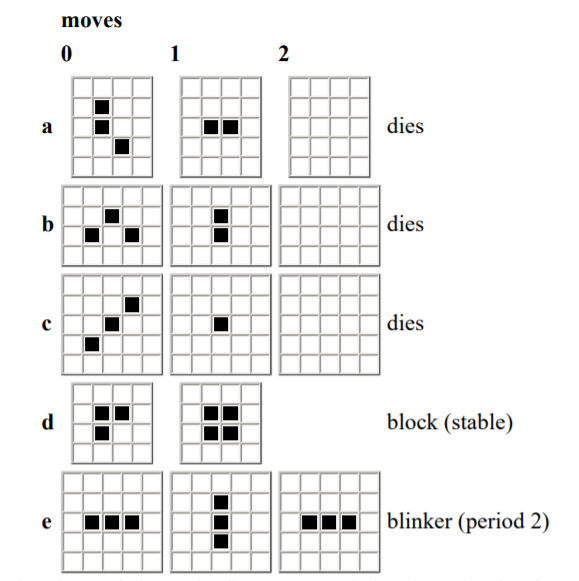
\includegraphics[width=\linewidth]{img/moves_1.png}
\caption{Evolution innerhalb von drei Generationen (entnommen aus \cite{gardner1970mathematical})}
\label{moves_1}
\end{figure}
In Abbildung \ref{moves_2} führen die Startmuster zu einem sogenannten "`beehive"', welches in dieser Position verharrt.
\begin{figure}[H]
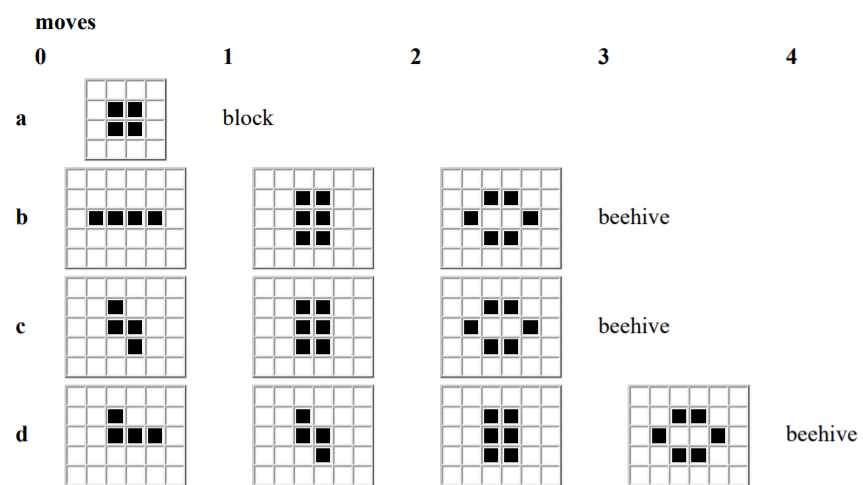
\includegraphics[width=\linewidth]{img/moves_2.png}
\caption{Evolution innerhalb von vier Generationen (entnommen aus \cite{gardner1970mathematical})}
\label{moves_2}
\end{figure}

\paragraph{Implementierung}

Für die Implementierung des Algorithmus wurden folgende Parameter gewählt:
\begin{itemize}
\item Anzahl der Spalten und Reihen des Gitters: Es wird eine Zahl angegeben, durch die die Weite und Breite des Gitters geteilt wird. So ergibt sich dann die Anzahl der Spalten und Reihen.
\item Farbe für den Vorgang der Reproduktion: Immer wenn eine Zelle geboren wird, wird sie für diese Runde in dieser Farbe angezeigt.
\item Farbe für den Vorgang des Sterbens: Immer wenn eine Zelle stirbt, wird sie für diese Runde in dieser Farbe angezeigt.
\end{itemize}
Wobei die Farbe für tote Zellen immer transparent und die Farbe für lebende Zellen immer schwarz ist. Die Startwerte für das Gitter werden anhand des vorhergehenden Algorithmus oder, sollte dies der erste Algorithmus sein, zufällig anhand eines Seeds gewählt. Nach dem Start beginnt das Spiel des Lebens und kann beispielsweise nachfolgende Bilder ergeben. Die nächsten vier Bilder zeigen die Evolution eines acht mal acht Gitter (hellblau = sterben, hellgrün = geboren werden). Die Bildschirmbreite und -höhe wurde bei 1000 Pixeln festgesetzt, welche wiederum durch 120 geteilt wurde, um die Spalten- bzw. Reihenanzahl zu erhalten.

\begin{figure}[H]

\includegraphics[width=5cm]{img/8x8_start.png}
\caption{Startzustand des 8x8-Gitters (eigene Darstellung)}
\label{8x8_start}
\end{figure}

\begin{figure}[H]

\includegraphics[width=5cm]{img/8x8_firstgen.png}
\caption{Die erste Generation (eigene Darstellung)}
\label{8x8_firstgen}
\end{figure}

\begin{figure}[H]

\includegraphics[width=5cm]{img/8x8_gen16.png}
\caption{16. Generation: Achsensymmetrisches (fast punktsymmetrisches) Objekt (eigene Darstellung)}
\label{8x8_gen16}
\end{figure}

\begin{figure}[H]

\includegraphics[width=5cm]{img/8x8_final.png}
\caption{Endzustand des 8x8-Gitters (eigene Darstellung)}
\label{8x8_final}
\end{figure}

Die nächsten fünf Bilder zeigen die Evolution eines 12 mal 12 Gitters (blau = sterben, grün = geboren werden), wobei diese Konfiguration zum Aussterben aller Zellen nach 45 Generationen führt. Die Bildschirmbreite und -höhe wurde bei 1000 Pixeln festgesetzt, welche wiederum durch 80 geteilt wurde, um die Spalten- bzw. Reihenanzahl zu erhalten.

\begin{figure}[H]

\includegraphics[width=5cm]{img/12x12_start.png}
\caption{Startzustand des 12x12-Gitters (eigene Darstellung)}
\label{12x12_start}
\end{figure}

\begin{figure}[H]

\includegraphics[width=5cm]{img/12x12_firstgen.png}
\caption{Die erste Generation (eigene Darstellung)}
\label{12x12_firstgen}
\end{figure}

\begin{figure}[H]

\includegraphics[width=5cm]{img/12x12_gen4.png}
\caption[Vierte Generation: Sechser Block]{Vierte Generation: Hier führt ein Sechser-Block zu einem beehive in der nächsten Generation (eigene Darstellung, vgl. Abbildung \ref{moves_2})}
\label{12x12_gen4}
\end{figure}

\begin{figure}[H]

\includegraphics[width=5cm]{img/12x12_beehive_gen5.png}
\caption{Fünfte Generation: Es entstand ein beehive (eigene Darstellung)}
\label{12x12_beehive_gen5}
\end{figure}

\begin{figure}[H]

\includegraphics[width=5cm]{img/12x12_empty_gen45.png}
\caption{Endzustand des 12x12-Gitters: Alle Zellen sind gestorben (eigene Darstellung)}
\label{12x12_empty_gen45}
\end{figure}

Nach etlichen Generationen endet nachfolgendes Game of Life in vier Blinkern. Es handelt sich um ein zehn mal zehn Gitter. Die Konfiguration kann den Beispielen im Konfigurator entnommen werden.

\begin{figure}[H]

\includegraphics[width=5cm]{img/10x10_blinker_seed10000.png}
\caption{10x10 Gitter: Blinker 1 (eigene Darstellung)}
\label{10x10_blinker_seed10000}
\end{figure}

\begin{figure}[H]

\includegraphics[width=5cm]{img/other_10x10_blinker_seed10000.png}
\caption{10x10 Gitter: Blinker 2 (eigene Darstellung)}
\label{other_10x10_blinker_seed10000}
\end{figure}

\paragraph{Bewertung}
Das Beobachten der Evolution mithilfe des Game of Life Algorithmus macht Spaß. Dabei lässt sich die Stärke des Algorithmus ebenso als seine Schwäche bezüglich der Kooperation benennen. Der Algorithmus braucht nicht unbedingt eine Kooperation um schöne Bilder zu erzeugen. Er ist in sich schon sehr vielfältig, was dazu führt dass viele unterschiedliche Bilder entstehen. Des Weiteren ist der Algorithmus zunächst einmal im Rahmen seines Gitters eingeschränkt, eine Erweiterung auf 3D oder andere geometrische Objekte wäre sicher spannend. Je nachdem, wie der Startzustand des Algorithmus ist, kann auch ein leeres Bild entstehen, sofern alle Zellen gestorben sind. Der Algorithmus lebt von seiner Ausführung und weniger von dessen Endzustand. Der GOL kann unter Umständen sehr lange laufen, oder auch nur kurz. 


\subsubsection{L-System}

Das Lindenmayer-System bzw. L-System wurde 1968 von einem Biologen desselben Namens eingeführt. Es handelt sich um eine mathematische Theorie über die Entwicklung von (oft pflanzlichen) rekursiven Systemen. Für ein L-System werden also Regeln benötigt, die zur Generierung der Systeme herangezogen werden. Ein einführendes Axiom verzeichnet den Beginn der Entwicklung und die Regeln werden dann rekursiv angewendet \cite{wiki2018lsystem}. Es werden demnach nachfolgende Teilaspekte benötigt:
\begin{itemize}
\item Alphabet: Definition der Zeichen, die erlaubt sind.
\item Axiom: Definition des Beginns des Systems.
\item Regelsatz: Vorgabe der Regeln, welche rekursiv angewandt werden.
\end{itemize}
Zur besseren Darstellung soll ein einfaches Beispiel herangezogen werden:
\begin{itemize}
\item Alphabet: A und B,
\item Axiom: A,
\item Regelsatz: Aus A wird AB, aus B wird BB.
\end{itemize}
In Tabelle \ref{tab:l-system-beispiel} wird die rekursive Entwicklung dargestellt.

\begin{table}[H]
\begin{tabular}{@{}|l|l|l|l|l|@{}}
\toprule
\textbf{Axiom} & \textbf{Gen1} & \textbf{Gen2} & \textbf{Gen3} & \textbf{...} \\ \midrule
A              & AB            & ABBB          & ABBBBBBB      & ...          \\ \bottomrule
\end{tabular}
\caption{Anhand des Regelsatzes wird das Axiom rekursiv erweitert.}
\label{tab:l-system-beispiel}
\end{table}

Es wird schnell klar, dass der Algorithmus ohne Abbruchbedingung unendlich weiter laufen würde bzw. nur durch die Rechenleistung begrenzt ist. Wie kann dieser Algorithmus nun für eine grafische Darstellung genutzt werden? 

\paragraph{Implementierung}
Zur grafischen Umsetzung, muss den Regelsätzen eine andere Bedeutung gegeben werden. Dem Benutzenden der grafischen Oberfläche sollen die Wahl des x- und y-Startpunktes sowie der Farbe und verschiedene Regelsätze zur Verfügung gestellt werden. Die Regelsätze orientieren sich an Ihren Erfindern und heißen im Einzelnen:
\begin{itemize}
\item Verästelung,
\item Koch,
\item Fractal,
\item Sierpinksi Gasket Triangle und
\item Überraschung.
\end{itemize}
Beispielhaft soll auf drei davon im Folgenden eingegangen werden. Zunächst wird die "`Verästelung"' beschrieben:
\begin{itemize}
\item Alphabet: F = ein Stück zeichnen, [ = abspeichern, ] = auslesen, + = Drehung gegen den Uhrzeigersinn, - = Drehung im Uhrzeigersinn (jeweils um 45°, bzw. abhängig vom Seed)
\item Axiom: F-F-F-F
\item Regelsatz: Aus "`F"' wird "`F[F]-F+F[--F]+F-F"'
\end{itemize}

In Abbildung \ref{veraestelung_gen5} wird eine besonders schöne Verästelung dargestellt. In Abbildung \ref{gespiegelter_baum_gen6} wird mit Spiegelung gearbeitet.
\begin{figure}[H]

\includegraphics[width=10cm]{img/veraestelung_gen5.png}
\caption{Fünfte Generation: Ein Baum und weitere Verästelungen (eigene Darstellung)}
\label{veraestelung_gen5}
\end{figure}

\begin{figure}[H]
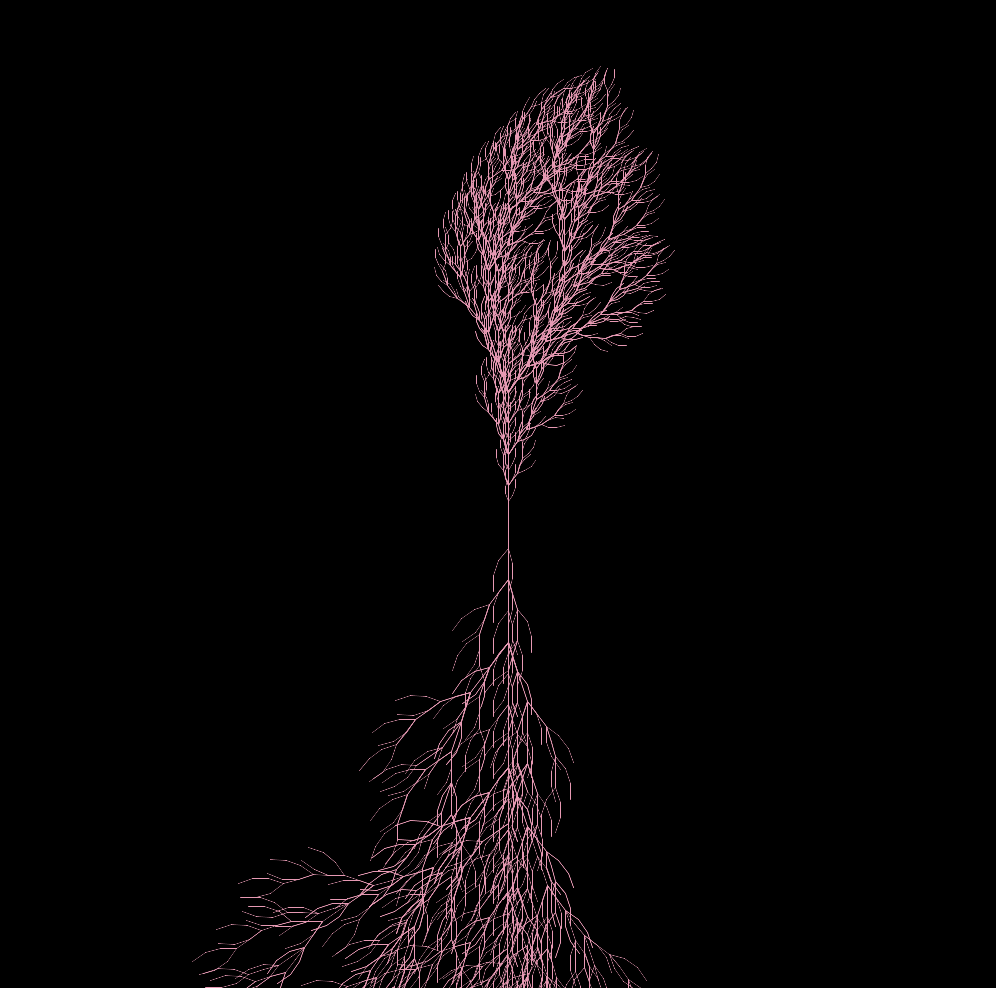
\includegraphics[width=10cm]{img/gespiegelter_baum_gen6.png}
\caption{Sechste Generation: Der Baum zeichnet abwechselnd nach oben und unten (eigene Darstellung)}
\label{gespiegelter_baum_gen6}
\end{figure}

Als zweite Kategorie der L-Systeme soll "`Fractal"' vorgestellt werden. 
\begin{itemize}
\item Alphabet: F = ein Stück zeichnen, + = Drehung gegen den Uhrzeigersinn, - = Drehung im Uhrzeigersinn (jeweils um 90°, bzw. abhängig vom Seed)
\item Axiom: F-F-F-F
\item Regelsatz: Aus "`F"' wird "`FF-F-F-F-F-F+F"'
\end{itemize}
Die Abbildungen \ref{fractal-gen5} bis \ref{fractal-gen5-grad} zeigen einige Fraktale. Fraktale sind natürliche oder künstliche, meist geometrische Muster, die eine gebrochene Hausdorff-Dimension besitzen. Daher kommt auch der Name. Sie weisen eine hohe Selbstähnlichkeit auf, wenn sie zum Beispiel aus kleineren Kopien von sich selbst bestehen \cite{mandelbrot1983fractal}. Der Algorithmus macht also viele kleinere Kopien von sich selbst und wird dabei um eine gewisse Gradzahl gedreht. Werden die Gradzahlen angepasst, können komplett unterschiedliche Bilder entstehen.

\begin{figure}[H]
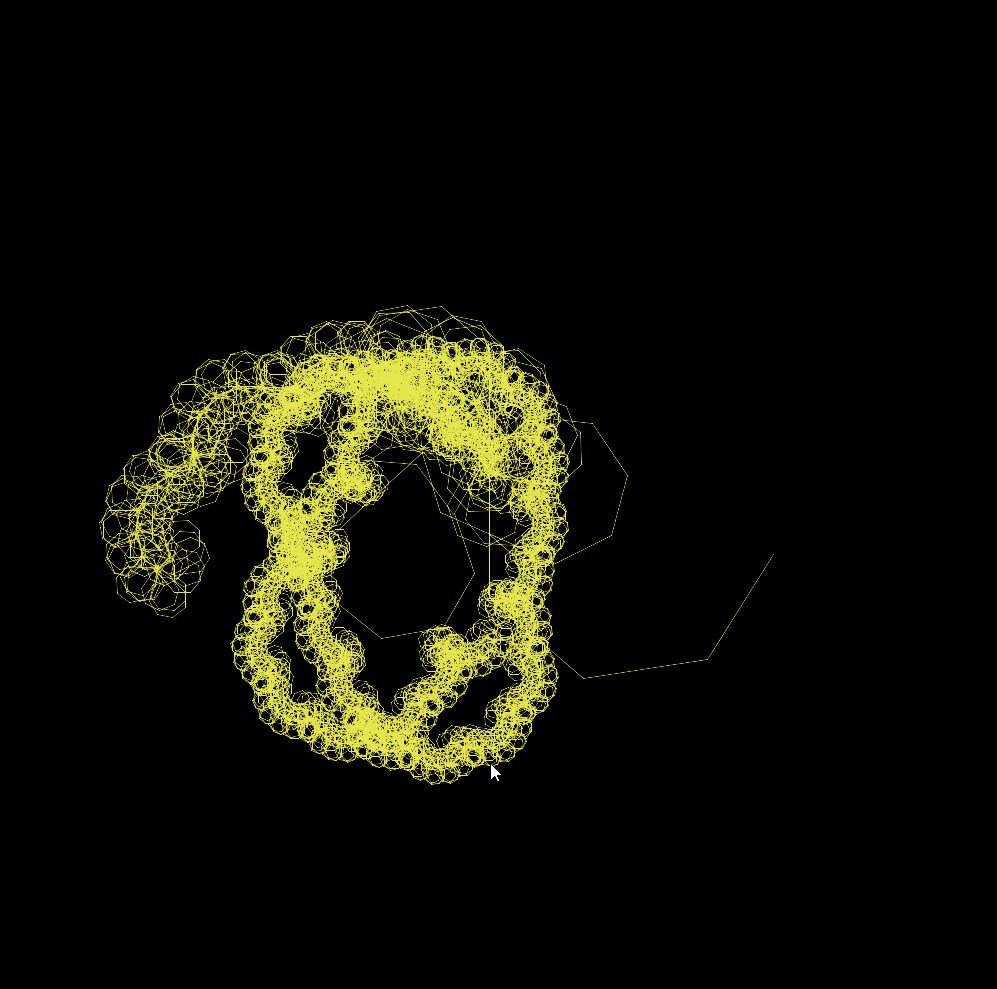
\includegraphics[width=10cm]{img/fractal-gen5.png}
\caption{Fünfte Generation: Eine wolkige Struktur (eigene Darstellung)}
\label{fractal-gen5}
\end{figure}

\begin{figure}[H]

\includegraphics[width=10cm]{img/fractal-gen6.png}
\caption{Sechste Generation: Die Fraktale sind fast über das gesamte Bild verteilt (eigene Darstellung)}
\label{fractal-gen6}
\end{figure}

\begin{figure}[H]
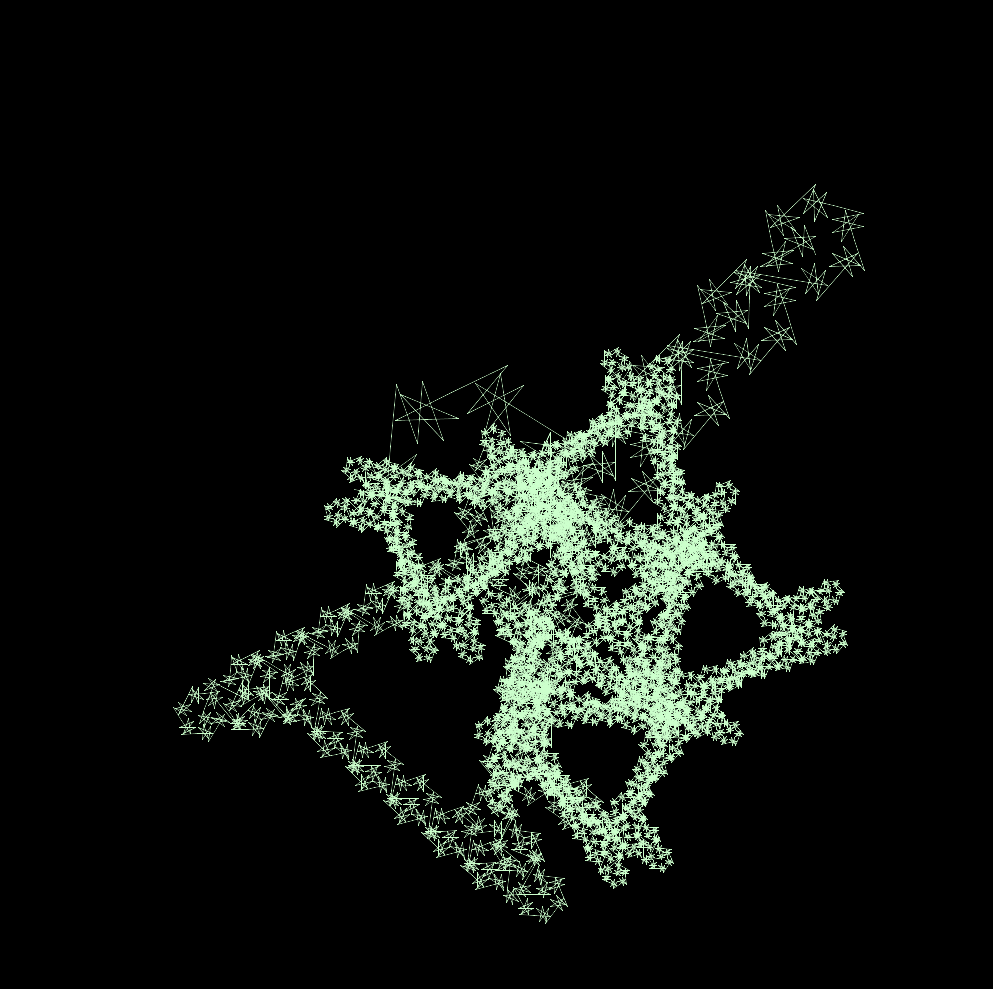
\includegraphics[width=10cm]{img/fractal-gen5-grad.png}
\caption[Fünfte Generation: Erhöhung der Gradzahl]{Fünfte Generation: Wird die Gradzahl erhöht, werden die Fraktale kantiger und erhalten eine Schneeflockenstruktur (eigene Darstellung)}
\label{fractal-gen5-grad}
\end{figure}

Zuletzt soll noch "`Sierpinski"' beschrieben werden. Hier enthält der Regelsatz zwei Regeln.
\begin{itemize}
\item Alphabet: F/G = ein Stück zeichnen, - = Drehung im Uhrzeigersinn (um 25°, bzw. abhängig vom Seed)
\item Axiom: F--F--F
\item Regelsatz: Aus "`F"' wird "`F--F--F--G"' und aus "`G"' wird "`GG"'
\end{itemize}

In den Abbildungen \ref{sierpinski-gen7} und \ref{sierpinski-gen10} wird "`Sierpinski"' in den Generationen sieben und zehn dargestellt. Der Algorithmus ist an der Sierpinski-Kurve orientiert.

\begin{figure}[H]
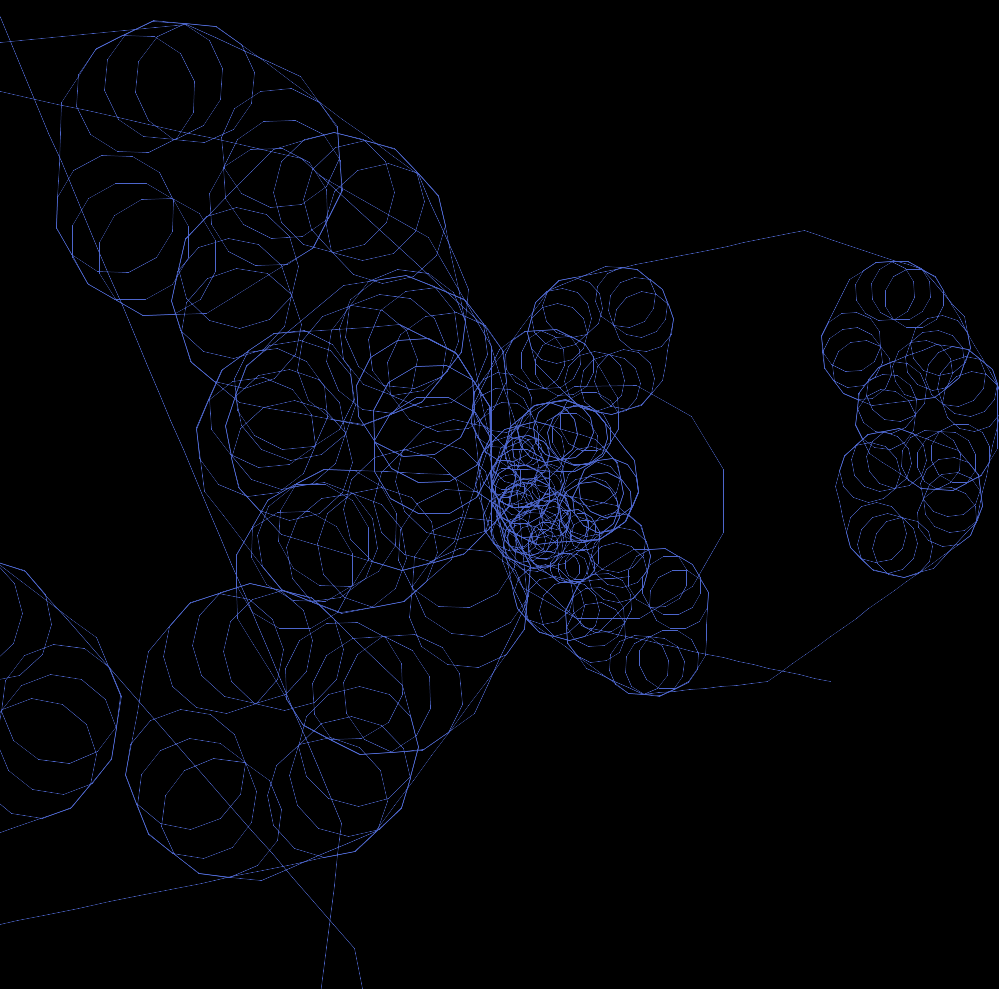
\includegraphics[width=10cm]{img/sierpinski-gen7.png}
\caption{Siebte Generation: Sieht einem Diamantring ähnlich (eigene Darstellung)}
\label{sierpinski-gen7}
\end{figure}

\begin{figure}[H]

\includegraphics[width=10cm]{img/sierpinski-gen10.png}
\caption{Zehnte Generation: Endlose Spiralen (eigene Darstellung)}
\label{sierpinski-gen10}
\end{figure}

\paragraph{Bewertung}
Der Algorithmus bietet unendlich viele Möglichkeiten, um verschiedene geometrische Formen darzustellen. Der Fantasie sind dabei keine Grenzen gesetzt. So gestaltet es sich auch mit der Kooperation. Ein Baum kann dort entstehen, wo ein vorheriges Bild geendet hat oder ein Schwarm kann aus den letzten Verästelungen eines Baumes heraus fliegen. Darüber hinaus ist ein L-System meistens selbst schon so komplex und beeindruckend, dass eine räumliche Kooperation, sprich nebeneinander gelegte Bilder auch für sich selbst stehen können.
Dadurch, dass L-Systeme zunächst nicht abbrechend sind und immer komplexer werden, kann es zu einem hohen Speicherverbrauch bzw. einer Runtime-Exception kommen. Die Iterationen sollten deshalb beschränkt sein.


\subsubsection{Particle System}
Mithilfe eines Partikelsystems lassen sich mehrere Objekte als Gesamtsystem animieren. Wind oder Feuer könnten solche Systeme sein oder beeinflussen. Durch verschiedene Parameter lassen sich die Partikel dann beeinflussen \cite{reeves1983particle}.


\paragraph{Implementierung}
Bei der Implementierung des Algorithmus diente \cite{shiffman2022smoke} als Vorlage. Es werden vier Bilder geladen (also durch den Nutzenden ausgewählt), welche dann von der Mitte des Bildes nach außen getrieben werden. Streng genommen handelt es sich also um vier Partikelsysteme. Das funktioniert, indem jeder neue Partikel der erstellt wird, die Optik des geladenen Bildes übernimmt. Die Windstärke wird vom vorherigen Algorithmus beeinflusst. Nach der Initialisierung der Systeme werden neue Partikel immer nur am Rand der Systeme hinzugefügt, zu dem der Wind sie treibt.
Beispiele können den Abbildungen \ref{black_materia_gen20} bis \ref{all_black} entnommen werden.

\begin{figure}[H]

\includegraphics[width=10cm]{img/black_materia_gen20.png}
\caption{20. Generation: Schwarze Materie (eigene Darstellung)}
\label{black_materia_gen20}
\end{figure}

\begin{figure}[H]

\includegraphics[width=10cm]{img/watercolor_gen20.png}
\caption{20. Generation: Wasserfarben werden über den Bildschirm verteilt (eigene Darstellung)}
\label{watercolor_gen20}
\end{figure}

\begin{figure}[H]

\includegraphics[width=10cm]{img/all_black.png}
\caption{Zehnte Generation: Die schwarzen Punkte verteilen sich (eigene Darstellung)}
\label{all_black}
\end{figure}

\paragraph{Bewertung}
Der Algorithmus hängt stark von den geladenen Bilder ab. Es ist daher von Vorteil, wenn ähnliche Bildstrukturen geladen werden, die auch ineinander verschwimmen können. Prinzipiell sind dadurch dem Erzeugen der Bilder und der Kreativität keine Grenzen gesetzt. 
Sofern der Algorithmus als erstes geladen wird, eignet er sich gut als Hintergrund für die darauffolgenden Algorithmen. Besonders nachfolgende Algorithmen, die anhand der vorherigen Farben beeinflusst werden funktionieren in dieser Verbindung gut. Räumliche Kooperationen funktionieren auch. Sollte der Algorithmus nicht als erstes geladen werden, überlagert er andere Bilder und eignet sich deshalb weniger. Nach etwa 30 Generationen wird der Speicherverbrauch relativ hoch. Die Iterationsanzahl sollte also begrenzt werden.

\subsubsection{Kooperation der eigenen Algorithmen}
Im Konfigurator lassen sich drei unterschiedliche Kooperationsmodi auswählen. Zunächst wird in Abbildung \ref{l_gol_p_l_gen5_nebeneinander} der Kooperationsmodus "`Nebeneinander 2x2"' dargestellt. Das Bild besteht von links oben nach rechts unten aus:
\begin{itemize}
\item LSystem: Fractal
\item Game of Life
\item Particle System
\item LSystem: Überraschung
\end{itemize}

\begin{figure}[H]
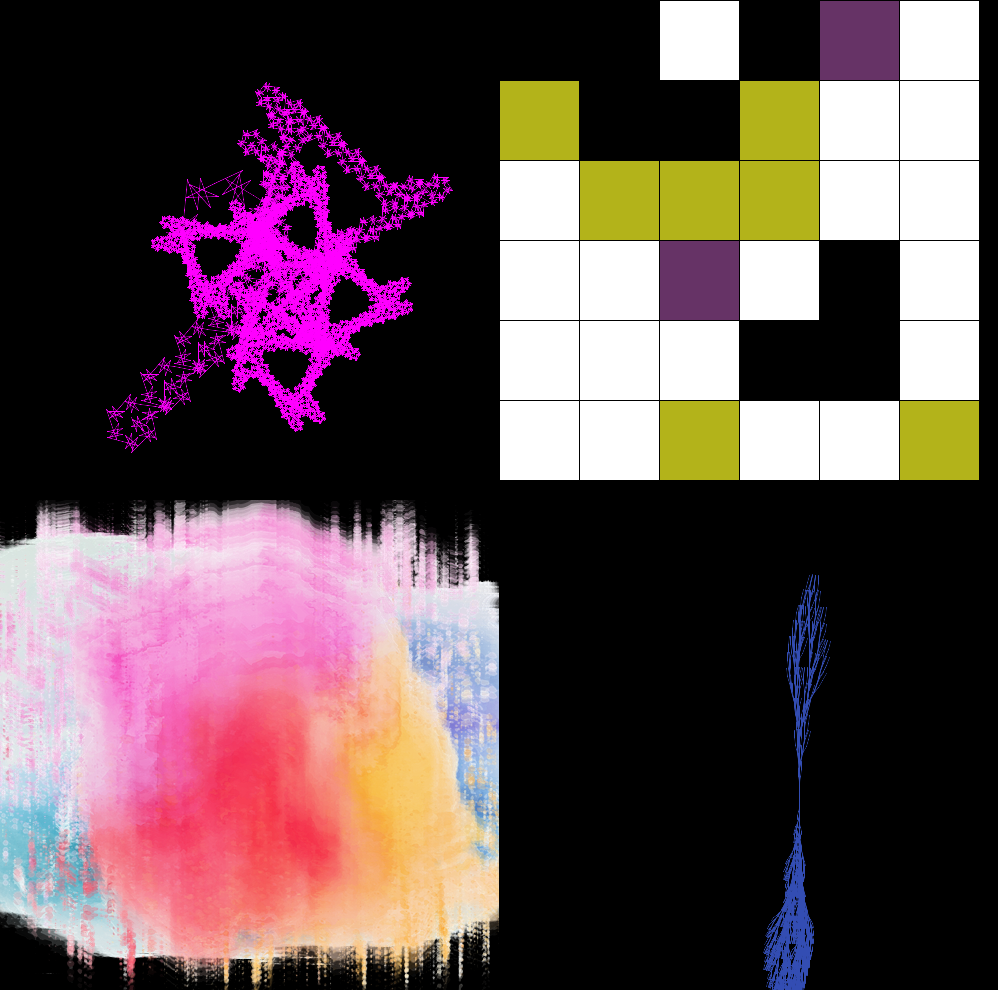
\includegraphics[width=\linewidth]{img/l_gol_p_l_gen5_nebeneinander.png}
\caption[Räumliche Trennung]{Fünfte Generation: Die vier Algorithmen werden räumlich getrennt voneinander ausgeführt (eigene Darstellung)}
\label{l_gol_p_l_gen5_nebeneinander}
\end{figure}

Als Nächstes wird in Abbildung \ref{sierpinski_veraestelung_gen8_nebeneinander2x1} der Kooperationsmodus "`Nebeneinander 2x1"' dargestellt. Das Bild besteht aus 2 L-Systemen: Sierpinski und Veraestelung.

\begin{figure}[H]

\includegraphics[width=\linewidth]{img/sierpinski_veraestelung_gen8_nebeneinander2x1.png}
\caption{Achte Generation: Die beiden L-Systeme entstehen nebeneinander (eigene Darstellung)}
\label{sierpinski_veraestelung_gen8_nebeneinander2x1}
\end{figure}

Zuletzt wird noch eine Kooperation "`Übereinander"' dargestellt. Für Abbildung \ref{materia_farctal_veraestelung_ueberraschung_uebereinander_gen5} wird zunächst das Partikelsystem geladen und dann werden drei L-Systeme darüber gelagert: Fractal, Verästelung und Überraschung.

\begin{figure}[H]
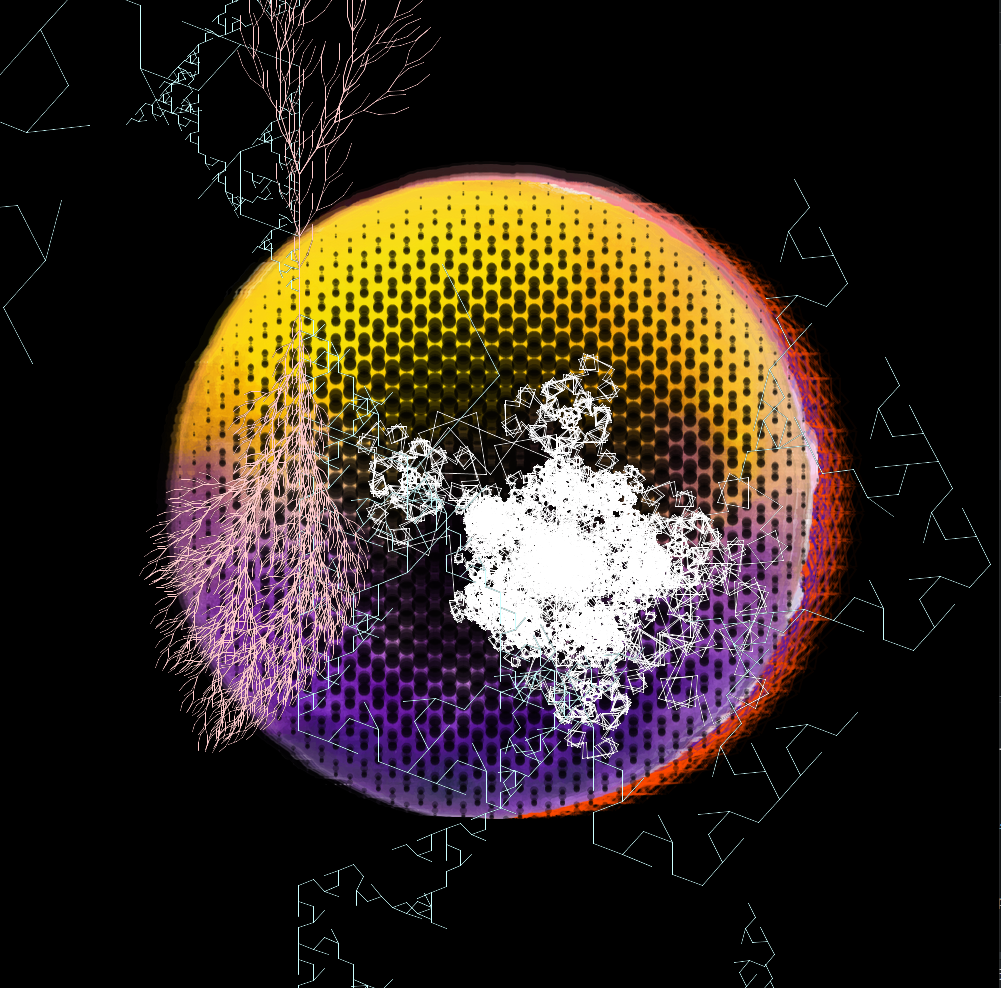
\includegraphics[width=\linewidth]{img/materia_farctal_veraestelung_ueberraschung_uebereinander_gen5.png}
\caption[Kooperation übereinander]{Fünfte Generation: Aus der schwarzen Materie heraus entstehen die beiden L-Systeme, dem Rand der Implosion entwächst ein Baum (eigene Darstellung)}
\label{materia_farctal_veraestelung_ueberraschung_uebereinander_gen5}
\end{figure}

%\bibliographystyle{babplain}
%\bibliography{../mciLiteratur}
\end{document}
			\subfile{ccamier/ccamier}
			\clearpage
		\subsection{Generatoren von Sabine Hopf}
			% \documentclass[../mciAusarbeitung.tex]{subfiles}

\usepackage[utf8]{inputenc}
\usepackage[T1]{fontenc}
\usepackage{lmodern}
\usepackage[german]{babel}
\usepackage[fixlanguage]{babelbib}
\selectbiblanguage{german}
\usepackage{amssymb}
\usepackage{graphicx}
\usepackage{url}
\usepackage{float}

\title{Fachpraktikum MCI (01513) - WS 2021/22}
\author{Gruppe 2\\
	Sabine Hopf}
\date{\today}

\begin{document}
	Es wurden Generatoren aus drei unterschiedlichen Kategorien implementiert, die nachfolgend beschrieben werden. Außerdem wird die Varianz der Generatoren und deren Kooperationsmöglichkeiten vorgestellt.\\
	\subsubsection{L-System}
		L-Systeme oder Lindenmayer-Systeme sind Systeme, die sich auf künstlerischer Ebene eignen, realitätsnahe Pflanzenmodellierungen oder andere Fraktale zu generieren. \\
		Das wesentliche Prinzip besteht darin, nach und nach einzelne Symbole mit entsprechenden Produktionsregeln durch andere Symbole zu ersetzen und dies bis zu einer Tiefe n rekursiv auszuführen. Durch eine sogenannte Turtle-Grafik werden dann die Symbole in entsprechende Linien oder Winkel transformiert.
		Dabei besteht das L-System aus einem Alphabet V aus Terminal- und Nichtterminalsymbolen, einem Startwort $\omega  $ aus dem Alphabet V und Produktionsregeln P, die festlegen, welche Nichtterminalsymbole durch welche Symbole oder Abfolge von Symbolen ersetzt werden sollen.\\
		Als Beispiel:\\
		\\
		n = 0\\
		$ \omega $ = F\\
		P = F->F[-F]\\
		Diese würde bei n = 1 bedeuten:\\
		F[-F]\\
		bei n = 2:\\
		F[-F][-F[-F]] usw.\\
		\\
		Die Visualisierung dieser Symbole wird nun so realisiert, dass man sich bildlich eine Schildkröte (daher Turtle-Grafik) vorstellt, die mit einem Stift über den Bildschirm läuft und an den entsprechenden Symbolen z. B. Linien zeichnet (hier z. B. beim 'F') und bei einem anderen Symbol (hier z. B. bei '-') die Richtung in einem bestimmten Winkel ändert. Durch einen LIFO-Speicher (Last In First Out) wird bei dem Symbol '[' der aktuelle Zustand, also die Position und Richtung der Schildkröte (bzw. das aktuelle Koordinatensystem) auf dem  Stack gespeichert und bei dem Symbol ']' der oberste Zustand vom Stack entfernt und zum aktuellen Zustand gemacht.\\
		L-Systeme können nicht nur für Pflanzenmodellierungen genutzt werden, sondern z. B. auch für Kochsche Schneeflocken und Drachenkurven.\\
		\paragraph{Beschreibung der Implementierung}$~$\\
		Die Implementierung erfolgte inspiriert von 'The nature of code' \cite{shiffman2012nature} wie oben beschrieben.
		Es wurden mit Hilfe der Produktregeln von 'The algorithmic beauty of plants'  \cite{prusinkiewicz2012algorithmic} S. 25, verschiedene Regeln für unterschiedliche Bäume implementiert.\\
		Die Regeln werden nach Auswahl des entsprechenden Baumes aus einem Rules-Array geladen und ausgeführt.\\
		Die Bäume sind parametrisierbar durch ihren Startpunkt in x und y Richtung, die Farbe der Zweige und der Anfangsrotation des Baumes. Außerdem kann die Anzahl der Bäume gewählt werden, im Bereich von 1 bis 10.\\
		Die Winkelgröße und die Länge der Zweige werden gegebenenfalls durch die Parameter der anderen Generatoren beeinflusst und können deshalb nicht individuell eingestellt werden. Außerdem entarten die Bäume, wenn der Zufallsparameter kleiner als 0,5 ist. Dieser Wert wurde willkürlich gewählt, um noch mehr Variationen zu erzeugen. Auch die Startpunkte und die Alphawerte der Bäume > 1 werden durch den Zufallsparameter beeinflusst. Gleichzeitig berechnet der Algorithmus noch einen Punkt, der im ersten Baum liegt, der von anderen Generatoren als Kooperation genutzt werden kann.\\
		Der Algorithmus benutzt seinerseits den Kooperationspunkt, um zu entscheiden, zu welcher Richtung manche Bäume gezeichnet werden. Ist die x-Koordinate des Kooperationspunktes größer als die halbe Weite des Zeichenfensters, wird der Baum zur jeweils anderen Seite als der normalen Seite ausgerichtet, außerdem variiert der Alpha-Wert der Farbe.\\
		
		\paragraph{Beispiele}$~$\\
		Unten wurde das Beispiel aus der Aufgabenstellung nachgebaut. Daneben wurde nur der x-Wert der Startposition über die Mitte des Bildes verschoben. Man kann erkennen, wie sich die Richtung des Baumes verändert hat, außerdem variiert der Alpha-Wert der Farbe:\\
		Bildgenerierung links:,,Menübar/Beispiele/SHopf/L-System/TreeBeispiel''\\
		Bildgenerierung rechts:,,Menübar/Beispiele/SHopf/L-System/TreeBeispielRichtung''\\
		\begin{figure}[H]
			\begin{minipage}[t]{0.45\linewidth} 
				
\includegraphics[width=\linewidth]{img/treeBeispiel.png}
				\caption[TreeBeispiel]{Beispiel aus Aufgabenstellung (eigene Darstellung)}
			\end{minipage}
			\hfill
			\begin{minipage}[t]{0.45\linewidth} 
				
\includegraphics[width=\linewidth]{img/treeRichtung.png}
				\caption[TreeBeispielRichtung]{Beispiel aus Aufgabenstellung mit verschobenem x-Wert (eigene Darstellung)}
			\end{minipage}
		\end{figure}
		\noindent Unten wurde die Anfangsrotation so weit gestellt, dass auch Abbildungen auf dem Kopf möglich sind:\\
		Bildgenerierung:,,Menübar/Beispiele/SHopf/L-System/TreeKopf''\\
		\begin{figure}[H]
			\centering
			
\includegraphics[width=0.5\linewidth]{img/treeKopf.png}
			\caption[TreeKopf]{Baum auf dem Kopf (eigene Darstellung)}
		\end{figure}
		\noindent Unten wurde die Anzahl der Bäume auf 10 gestellt. Hier kann man noch mal alle Variationen erkennen, wie die Bäume die Richtung ändern und der Alphawert variiert:\\
		Bildgenerierung:,,Menübar/Beispiele/SHopf/L-System/TreeRichtung''\\
		\begin{figure}[H]
			\centering
			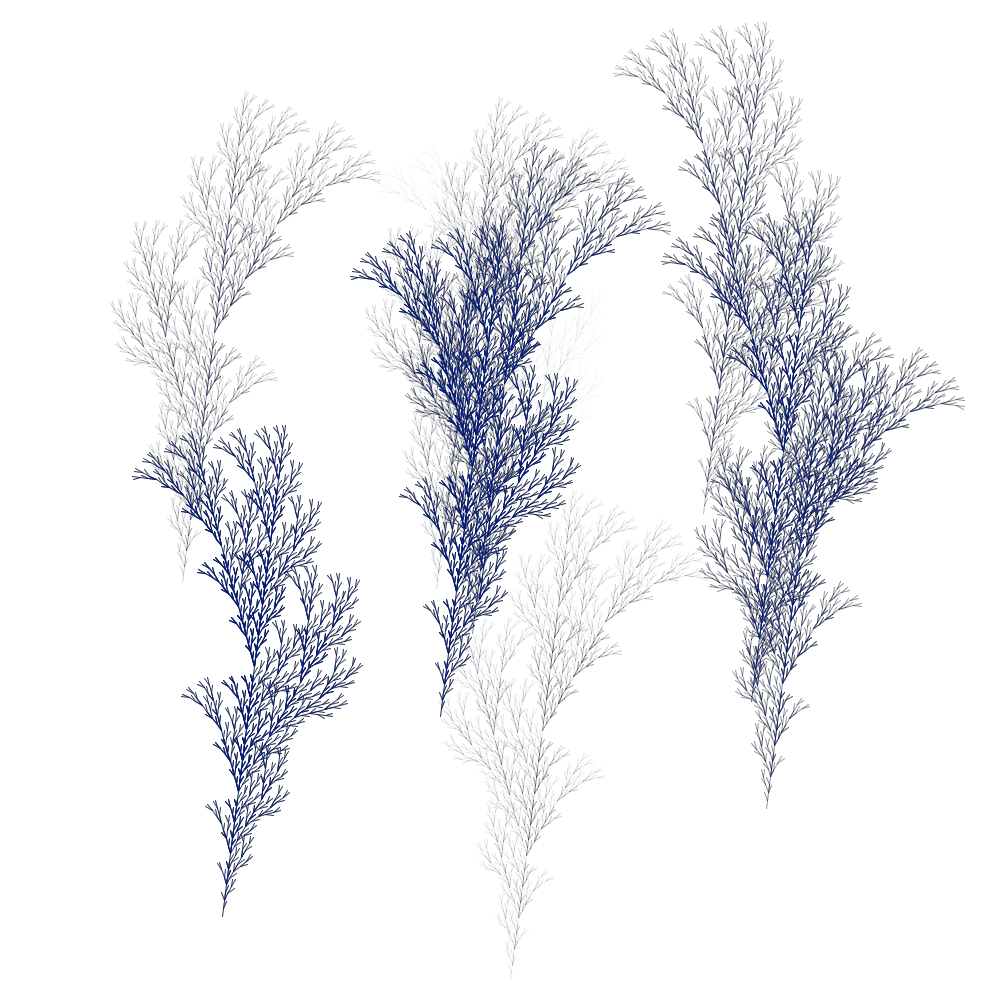
\includegraphics[width=0.5\linewidth]{img/tree10Richtung.png}
			\caption[TreeRichtung]{10 Bäume Variation (eigene Darstellung)}
		\end{figure}
		\noindent Unten wurden nochmal alle Bäume kombiniert. Man kann sehen, dass zu den anderen Variationen noch hinzu kommt, dass Bäume entarten und sich die Größe der Bäume unterscheidet:\\
		Bildgenerierung:,,Menübar/Beispiele/SHopf/L-System/TreeKombi''\\
		\begin{figure}[H]
			\centering
			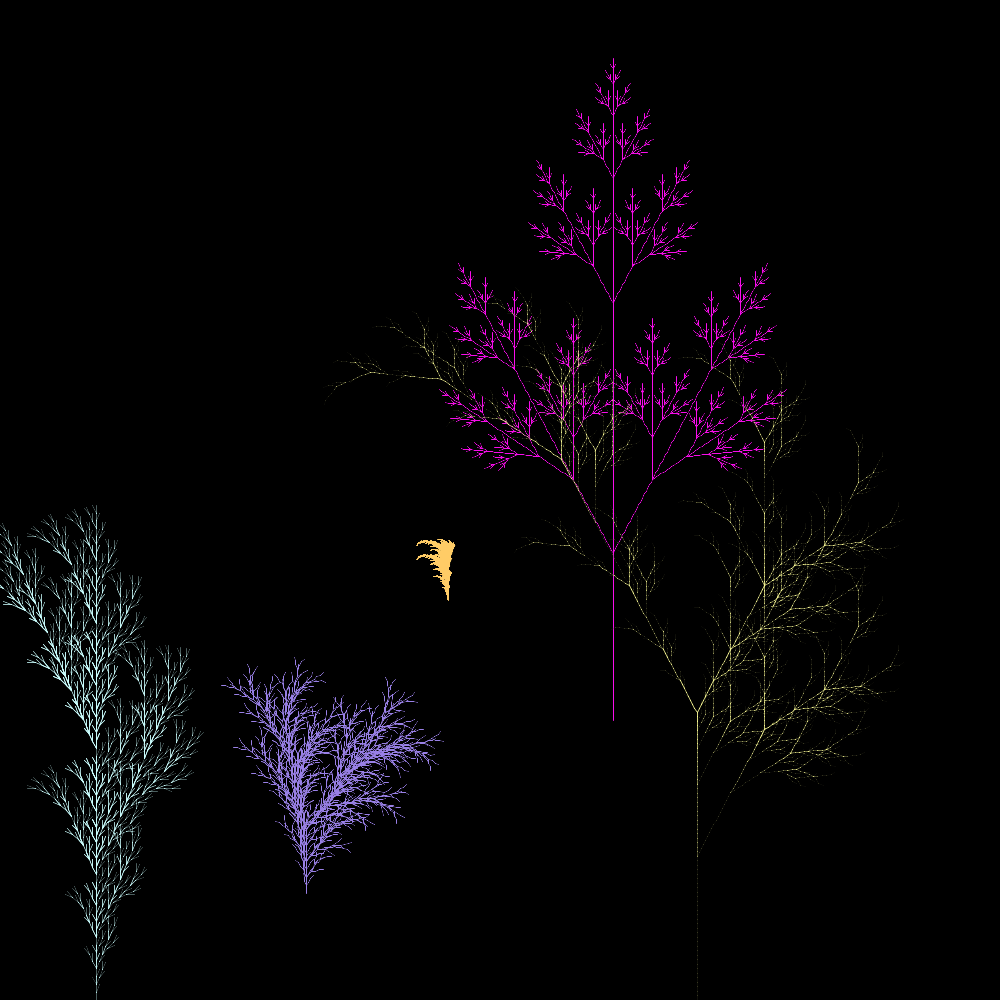
\includegraphics[width=\linewidth]{img/treeKombi.png}
			\caption[TreeKombi]{Verschiedene Bäume Variationen (eigene Darstellung)}
		\end{figure}
		
				
		
		\paragraph{Stärken und Schwächen}$~$\\
		Die Stärken des L-Systems liegen sicherlich darin, dass mit einem relativ einfachen Algorithmus erstaunlich komplexe Gebilde erschaffen werden können. Auf der anderen Seite darf die Rekursionstiefe $ n $ speziell bei den Bäumen nicht zu hoch sein, da sonst der Speicherplatz exponentiell wächst.\\
		Der Algorithmus ist auf jeden Fall für die Einzelgenerierung geeignet, da man dort Größe und Ausrichtung des Baumes auf die Größe des Bildes und den Geschmack des Betrachters ausrichten kann. Bei der Kooperation ist dies nicht unbedingt gegeben. Der Winkel der Zweige kann so klein werden, dass nur noch ein Strich übrig bleibt. Der Baum kann auch so klein werden, dass er fast nicht mehr gesehen wird, oder so groß, dass er nicht mehr ins Bild passt. Vielleicht kann aber auch dieser Zufall gerade den Reiz des Bildes ausmachen.
	 
	 
	\subsubsection{Simulation von Schwarmverhalten}
		Synchronisiertes Gruppenverhalten in Herden oder Schwärmen, egal ob von Fischen, Vögeln oder Säugetieren sind die Vorlage für diesen Algorithmus. Dabei kann man leicht vermuten, dass es bei diesem Verhalten einen Anführer geben muss, der die anderen Gruppenmitglieder auf irgendeine Art und Weise anleitet oder führt. Es deutet aber alles darauf hin, dass die gemeinsame Bewegung ein summiertes Verhalten der einzelnen Individuen sein muss.\\
		Craig Reynolds beschreibt in seinem Artikel ,,Flocks, Herds, and Schools: A Distributed Behavioral Model'' \cite{reynolds1987flocks} einen einfachen Ansatz ein Schwarmverhalten zu simulieren. Angelehnt an ein Particle-System, bei dem eine große Ansammlung einzelner Teilchen jeweils ein eigenes Verhalten hat, hat er seine sogenannten ,,Boids'' erschaffen. Diese haben jeweils ein eigenes Verhalten, welches er auf drei Steuerungsmechanismen reduziert. Alignment, Cohesion und Separation.
		\begin{itemize}
			\item Alignment steht dabei für Ausrichtung auf den durchschnittlichen Kurs der anderen
			\item Cohesion steht dabei für Zusammenhalt bezüglich der durchschnittliche Position der anderen
			\item Separation steht dabei für Trennung, d. h. ein gewisser Abstand, bzw. Freiraum zu den anderen
		\end{itemize}
		Jeder Boid reagiert nur auf die Geschehnisse in seiner Nachbarschaft. Hier kann also ein bestimmter Radius eingestellt werden, in dem ein Boid die anderen Boids ,,sieht''. Auch dies ist dem Wahrnehmungskreis der Individuen in der Natur nachempfunden, z. B. wenn Fische im trüben Wasser schwimmen.
		\paragraph{Beschreibung der Implementierung}$~$\\
		Die Implementierung erfolgte inspiriert von 'The nature of code' \cite{shiffman2012nature} wie oben beschrieben.
		Zuerst werden die Boids erstellt. Die Anzahl der Boids sind parametrisiert und können im Bereich von 1 bis 1000 gewählt werden. Außerdem ist auch das Aussehen der Boids parametrisiert und der Benutzer hat die Auswahl zwischen Punkten, Kurven und Dreiecken. Die Boids werden zunächst zufallsmäßig auf dem Bildschirm verteilt. Dieser Zufall wird allerdings im ganzen Algorithmus, bzw. in allen Generatoren durch Pseudozufallszahlen ermittelt, die durch einen seed inititalisiert werden. Damit ist sichergestellt, dass die Bildgenerierung deterministisch bleibt.\\
		Weiterhin erhält jeder Boid eine zufällige Geschwindigkeit und eine zufällige Farbe aus dem Regenbogenspektrum. Dann berechnet jeder Boid die durchschnittliche Ausrichtung der anderen Boids in seinem Wahrnehmungskreis und lenkt dementsprechend in diese Richtung. Genauso lenkt er sich in die durchschnittliche Position mit gleichzeitiger Wahrung des Abstandes zu den anderen Boids. So entstehen immer wieder kleinere Gruppen, die das Schwarmverhalten simulisieren.\\
		Als Besonderheit in diesem Algorithmus nehmen die Boids die Farbe ihrer Nachbarn im Wahrnehmungskreis an. Wenn sie sich von der Gruppe entfernen, nehmen sie wieder ihre Originalfarbe an.\\
		Als weitere Parametrisierung kann die Wahrung des Abstandes zu anderen Boids eingestellt werden. Damit noch andere Kräfte auf den Schwarm wirken, enthält der Algorithmus noch ein Hindernis, bei dem der Benutzer die Stärke der Abwehrkraft einstellen kann. Diese bewirkt, dass die Boids dieses Hindernis meiden. Das Hindernis kann wahlweise sichtbar oder unsichtbar eingestellt werden.\\
		Dadurch, dass ein Boid nur die anderen Boids in seinem Wahrnehmungskreis berechnen muss, ist der Algortihmus etwas effektiver, als wenn er alle Boids auf der gesamten Zeichenfläche berechnen müsste. Möglich macht dies die Einbindung eines Quadtrees, bei dem die Zeichenfläche zunächst in vier Quadrate unterteilt wird. In jedem Quadrat dürfen sich höchstens vier Boids aufhalten. Werden es mehr, teilt sich das Quadrat wieder in vier Quadrate usw. Dies wird rekursiv ausgeführt. Auch der Quadtree kann wahlweise sichtbar oder unsichtbar eingestellt werden, aus künstlerischen Gründen, aber auch wenn man diesen einfach mal in Aktion sehen möchte.\\
		Die Kooperation mit anderen Generatoren erfolgt einerseits mit den pseudozufallsmäßigen Variablen, die die Startpositionen der Boids und die Anfangsgeschwindigkeit beeinflussen, da der Seed durch die Parametrisierung aller beteiligten Generatoren beeinflusst wird. Auf der anderen Seite kann der Standort des Hindernisses von anderen Generatoren beeinflusst werden, wenn diese ein Interface benutzen, in dem sie diesen Punkt berechnen.\\
		Der Algorithmus gibt seinerseits den Standort des Hindernisses als Kooperationspunkt weiter.\\
		
		\paragraph{Beispiele}$~$\\
		Unten sieht man 850 Boids in der Gestalt von Kurven mit Hindernis:\\
		Bildgenerierung:,,Menübar/Beispiele/SHopf/Schwarm/SchwarmKurven''\\
		\begin{figure}[H]
			\centering
			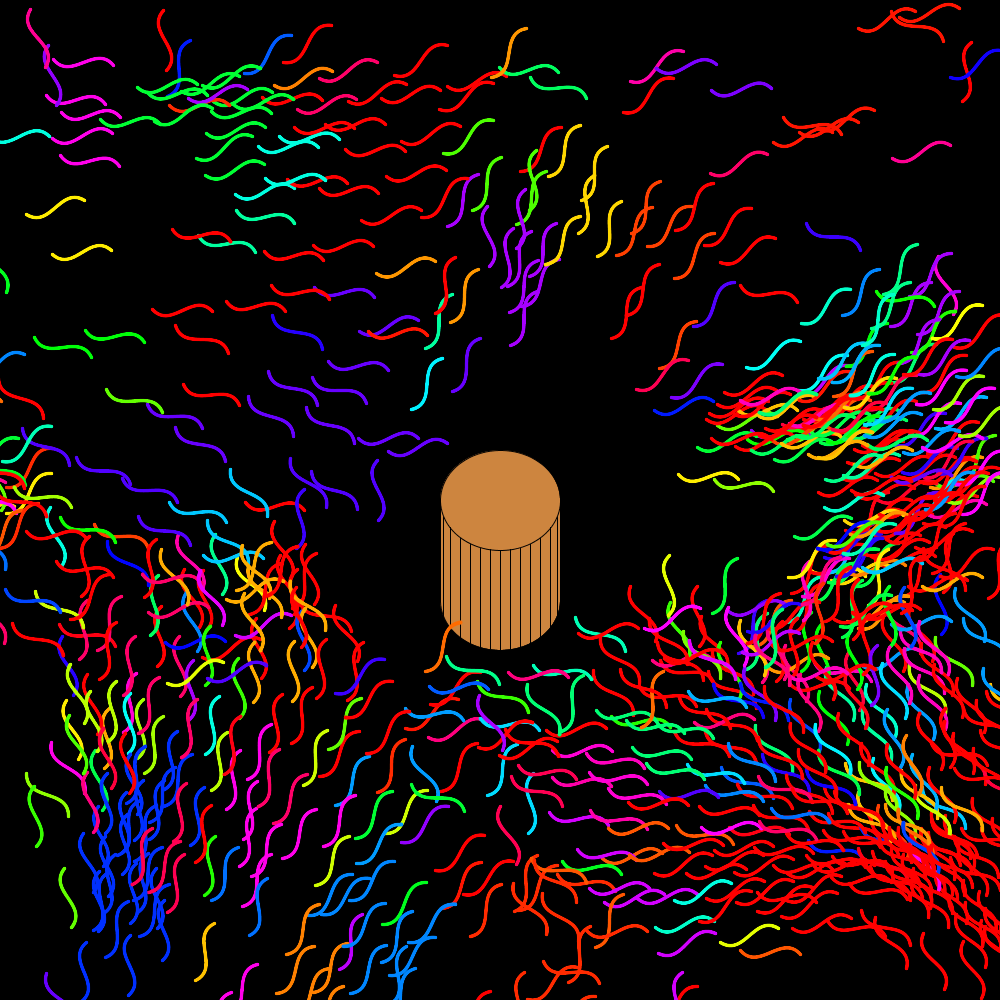
\includegraphics[width=0.5\linewidth]{img/schwarmKurven.png}
			\caption[SchwarmKurven]{Schwarm mit 850 Individuen und Hindernis (eigene Darstellung)}
		\end{figure}
		\noindent Unten wurde die Separation der Boids auf 5 gestellt. Damit wurde eine Verklumpung der Schwarmgruppen erreicht. Man kann gut erkennen, dass zwar das Hindernis nicht sichtbar geschaltet ist, dieses aber trotzdem den Abwehrmechanismus ausgelöst hat. Hier kann man weiterhin sichtbar machen, wie der Quadtree arbeitet. Es gibt viele kleine Quadrate an den Verklumpungen und nur große Quadrate, wo sich keine Boids aufhalten.\\
		Bildgenerierung:,,Menübar/Beispiele/SHopf/Schwarm/SchwarmQuad''\\
		\begin{figure}[H]
			\centering
			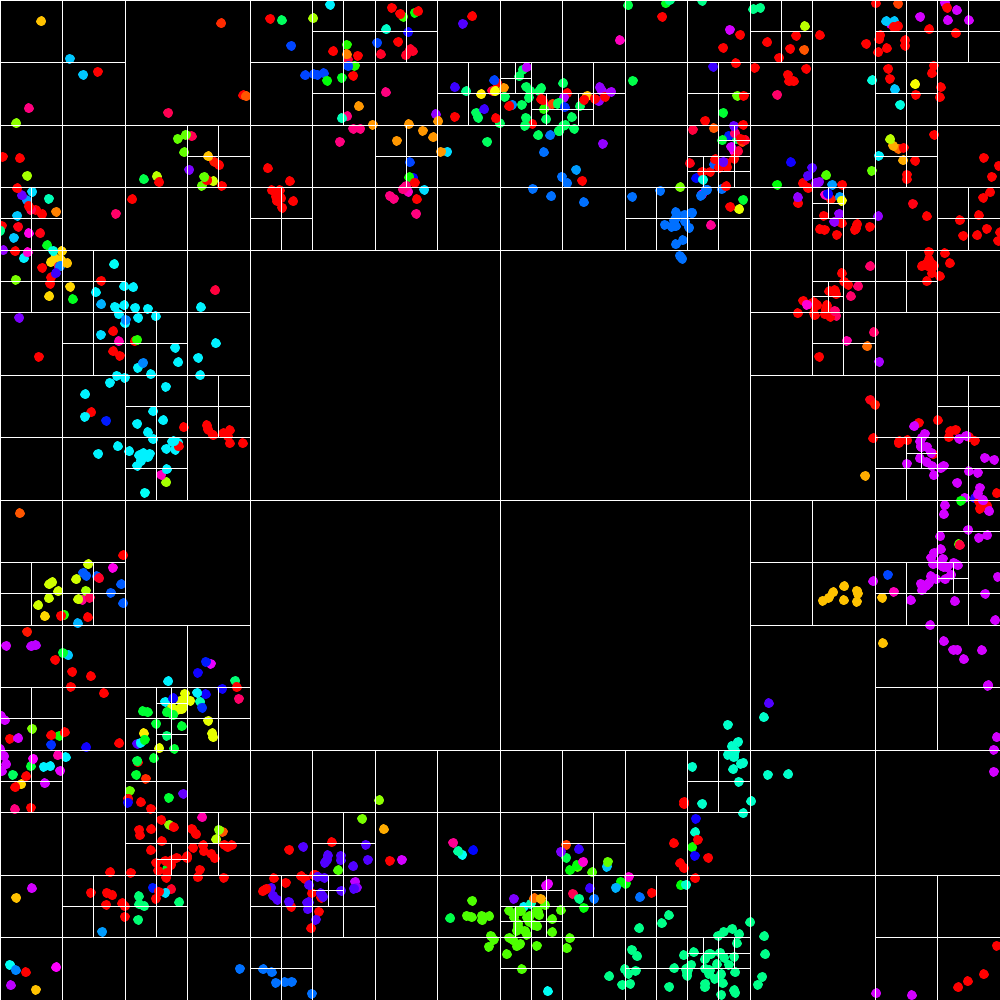
\includegraphics[width=0.5\linewidth]{img/schwarmQuad.png}
			\caption[SchwarmQuad]{Schwarm mit Separation 5 und Quadtree (eigene Darstellung)}
		\end{figure}
		\noindent Unten wurde der Verlauf der Kurven-Boids ausgeschaltet. Dadurch, dass diesmal die Separation der Boids auf 100 geschaltet wurde, versucht jedes Individuum möglichst allein für sich zu ,,schwimmen''. Dadurch ergeben sich schöne Verläufe.\\
		Bildgenerierung:,,Menübar/Beispiele/SHopf/Schwarm/SchwarmKunst''\\
		\begin{figure}[H]
			\centering
			
\includegraphics[width=0.5\linewidth]{img/schwarmKunst.png}
			\caption[SchwarmKunst]{Schwarm mit ausgeschaltetem Verlauf (eigene Darstellung)}
		\end{figure}
		
		
		\paragraph{Stärken und Schwächen}$~$\\
		Auch hier ist es faszinierend zu sehen, wie mit einem relativ einfachen Algorithmus ein Schwarmverhalten nachempfunden werden kann.\\
		Eine Schwäche liegt in der Laufzeit des Algorithmus. Wenn jeder Boid seine Position zu jedem anderen Boid prüfen muss, ergibt sich eine Laufzeit von O($ n^2 $). Der Quadtree bringt mehr Geschwindigkeit. Die Laufzeit kann auf O($ n \: log(n) $) verbessert werden, aber dadurch, dass dieser jedes Mal neu berechnet wird, wirkt sich dies erst richtig positiv bei großen Schwärmen aus.\\
		Der Algorithmus ist gut für die Einzelgenerierung geeignet. Man kann hier schon beeindruckende Bilder erhalten, erst recht, wenn man den Verlauf ausschaltet und die Punkte oder Kurven ihre Bahnen auch optisch ziehen.\\
		Auch bei der Kooperation kann man effektvolle Bilder erhalten. Hier kann man durch das ausgeschaltete Hindernis den Blick auf andere Bildelemente freihalten. Mit ausgeschaltetem Verlauf, ist der Schwarm eher für den Hintergrund geeignet. Auch sollte dann nur eine relativ kurze Iteration gewählt werden.\\
		
		\subsubsection{Evolutionärer Algorithmus}
		Auch für diesen Algorithmus liegt die Vorlage in der Biologie. Objekte sollen durch Evolution optimiert werden. Wie in der Natur gibt es eine Elterngeneration, die sich fortpflanzt und mit Hilfe der drei Schritte:
		\begin{itemize}
			\item Selection
			\item Crossover
			\item Mutation
		\end{itemize}
		die nächste Kindgeneration erschafft. Diese entwickelt sich im besten Fall näher auf ein Ziel zu. Danach wird diese Kindgeneration zur nächsten Elterngeneration usw.\\
		Der Algorithmus funktioniert so, dass zufällig generierte Objekte ein bestimmtes Ziel erreichen sollen, welches vorher definiert wurde. (Diese Ziele können z. B. sein: nimm eine bestimmte Farbe, eine bestimmte Richtung, eine bestimmte Form etc. an) Wie die Objekte dieses Ziel erreichen, wird aber nicht bestimmt. Es wird nur eine Fitnessfunktion geliefert, die die Objekte, die dieses Ziel zufällig erreicht haben, fitter machen. Durch die höhere Fitness der Individuen gelangt eine größere Anzahl von diesen Objekten, als von den weniger erfolgreichen Individuen (die Stärkeren überleben) in einen Paarungspool. Aus diesem Paarungspool werden dann zwei Elternteile gezogen (Selection), die durch Kreuzung (Crossover) neue Kinder für den Kinderpool erzeugen.
		Um die Vielfalt zu bewahren, werden zu einem geringen Prozentsatz auch wieder zufällige Objekte generiert (Mutation), die mit im neuen Kinderpool landen. Hieraus wird wieder der Elternpool und die Entwicklungs setzt sich fort bis der Algorithmus beendet und somit ein Ergebnis geliefert wird. (vgl. \cite{house2016autonomous})\\
		\paragraph{Beschreibung der Implementierung}$~$\\
		Die Implementierung erfolgte inspiriert von 'The nature of code' \cite{shiffman2012nature} wie oben beschrieben.
		Die Idee der Implementierung ist, dass eine Menge von Schnüren, die an einer bestimmten Stelle starten und eine zufällige Richtung, Farbe und Geschwindigkeit haben, sich auf ein Ziel ausrichten. Gleichzeitig behalten die Schnüre, die das Ziel erreichen ihre Farbe, so dass sich nach mehreren Generationen die Farben der Schnüre, die das Ziel erreichen, angleichen, bzw. im besten Fall übereinstimmen.\\
		Der Benutzer kann keinen Einfluss auf diese Evolution nehmen, sondern der Algorithmus arbeitet autonom. Die Anzahl der Schnüre und deren Startposition ist parametrisiert. Außerdem kann die Lebenszeit der Schnüre vom Benutzer eingestellt werden. Dies ist die Zeit, die den Schnüren bleibt, um ihr Ziel zu erreichen. Ist diese z. B. zu kurz, können sie zwar ihr Ziel nie erreichen, trotzdem wird die Ausrichtung aber nach einer gewissen Zeit in die Richtung des Ziel zeigen, da die Distanz des Schnurendes zum Ziel als Fitnesswert in die Berechnung einfließt. Durch die Evolution wird also auch hier den Schnüren, die sich auf das Ziel ausrichten der Vorzug gegeben.\\
		Inspiriert von ,,Autonomous Evolution of Digital Art Using Genetic Algorithms'' \cite{house2016autonomous} wurde noch eine Zielscheibe implementiert. Für die Viertelkreise etc. wurde ,,Processing - A Programming Handbook for Visual Designers and Artists'' \cite{reas2007processing} zu Hilfe genommen.\\ Hier hat der Benutzer nun die Möglichkeit zu wählen, wie viele Schnüre das Ziel treffen müssen, bevor sich die anfangs bunte Zielscheibe in eine einfarbige Scheibe verwandelt. Diese Verwandlung geschieht nach und nach, je nachdem wie viele Schnüre das Ziel schon getroffen haben, dabei färbt sich die Scheibe von innen nach außen gegen den Uhrzeigersinn einfarbig.\\
		Die Schnüre bilden sich aus Punkten, die sich auf dem Bildschirm bewegen. Dabei hat jede Schnur eine eigene DNA, die aus einer Farbe und einem  Vektor besteht, der dem Punkt eine Position, eine Richtung und eine Beschleunigung gibt.  Nachdem die Lebensspanne der Schnüre abgelaufen ist, wird die Fitness der Schnüre errechnet. Diese Funktion liefert die Distanz der Schnurenden zum Ziel. Um die Entwicklung noch zu beschleunigen, werden Schnüre, die eine Distanz unter 15 zum Ziel haben noch extra belohnt. Wie oben beschrieben landen Schnüre mit größerer Fitness in größerer Anzahl im nächsten Pool. Aus diesem Pool werden dann zufällig zwei Elternteile gezogen. Die Elternteile werden aber in diesem Algorithmus nicht gekreuzt, sondern es wird nur wiederum zufällig ein Elternteil als neues Kind gewählt. Diese Entwicklung wird so lange fortgesetzt, bis der Benutzer das Bild stoppt.\\
		Die Kooperation mit anderen Generatoren erfolgt auch hier mit den pseudozufälligen Variablen, die die Farbe und den Vektor initialisieren. Auch kann der Standort des Ziels von anderen Generatoren beeinflusst werden, wenn diese ein Interface benutzen, in dem sie diesen Punkt berechnen.\\
		Der Algorithmus gibt seinerseits den Standort der Schnüre als Kooperationspunkt weiter.\\
		
		\paragraph{Beispiele}$~$\\
		Unten kann man sehen, wie sich die Evolution unter den eingestellten Defaultwerten entwickelt. Nach 2100 Iterationen sieht man, dass mindestens 32 Schnüre die Zielscheibe getroffen haben und sich die Richtung der Schnüre eindeutig zum Ziel neigt. Die Farben haben sich vorrangig den lila Tönen angeglichen.\\
		Bildgenerierung links:,,Menübar/Beispiele/SHopf/Evolution/EvoDefault''\\
		Bildgenerierung rechts:,,Menübar/Beispiele/SHopf/Evolution/EvoDefaultEnd''\\
		\begin{figure}[H]
			\begin{minipage}[t]{0.45\linewidth} 
				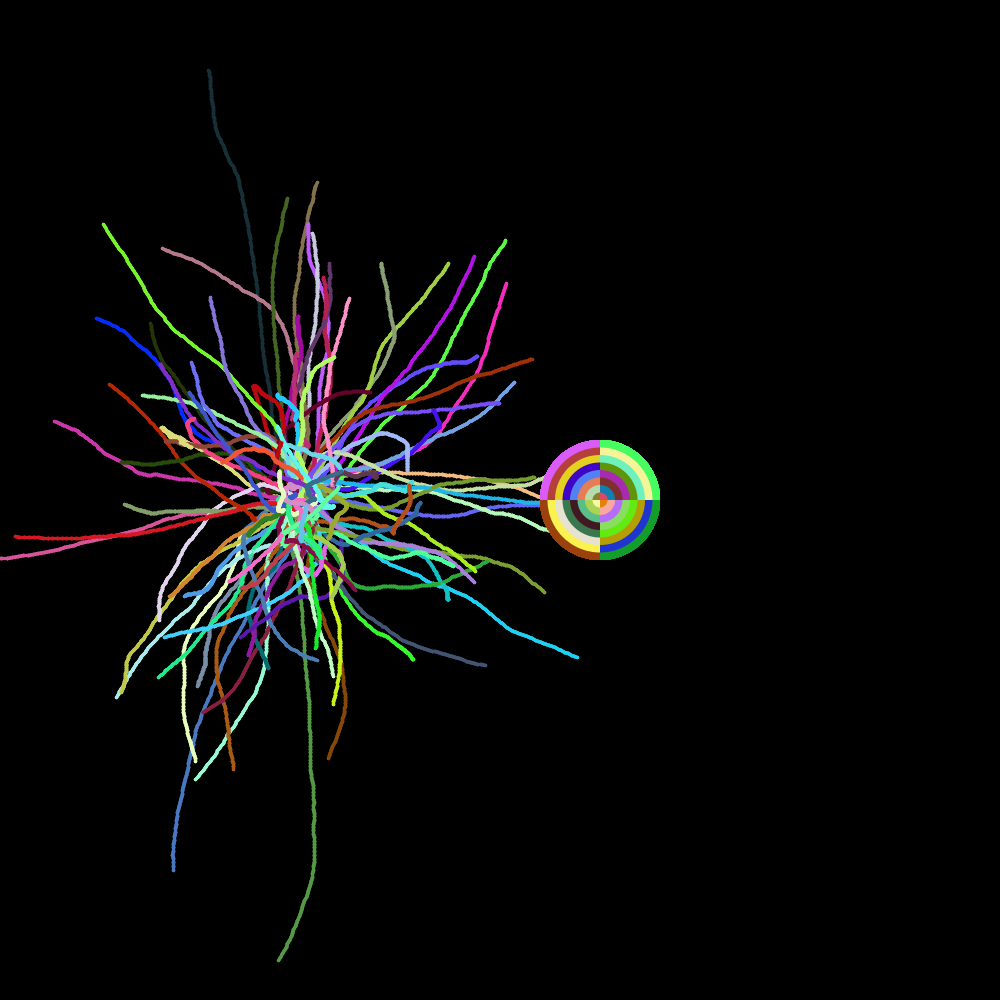
\includegraphics[width=\linewidth]{img/evoDefault.png}
				\caption[EvoDefault]{Evolution mit Defaultwerten nach 150 Iterationen (eigene Darstellung)}
			\end{minipage}
		\hfill
			\begin{minipage}[t]{0.45\linewidth} 
				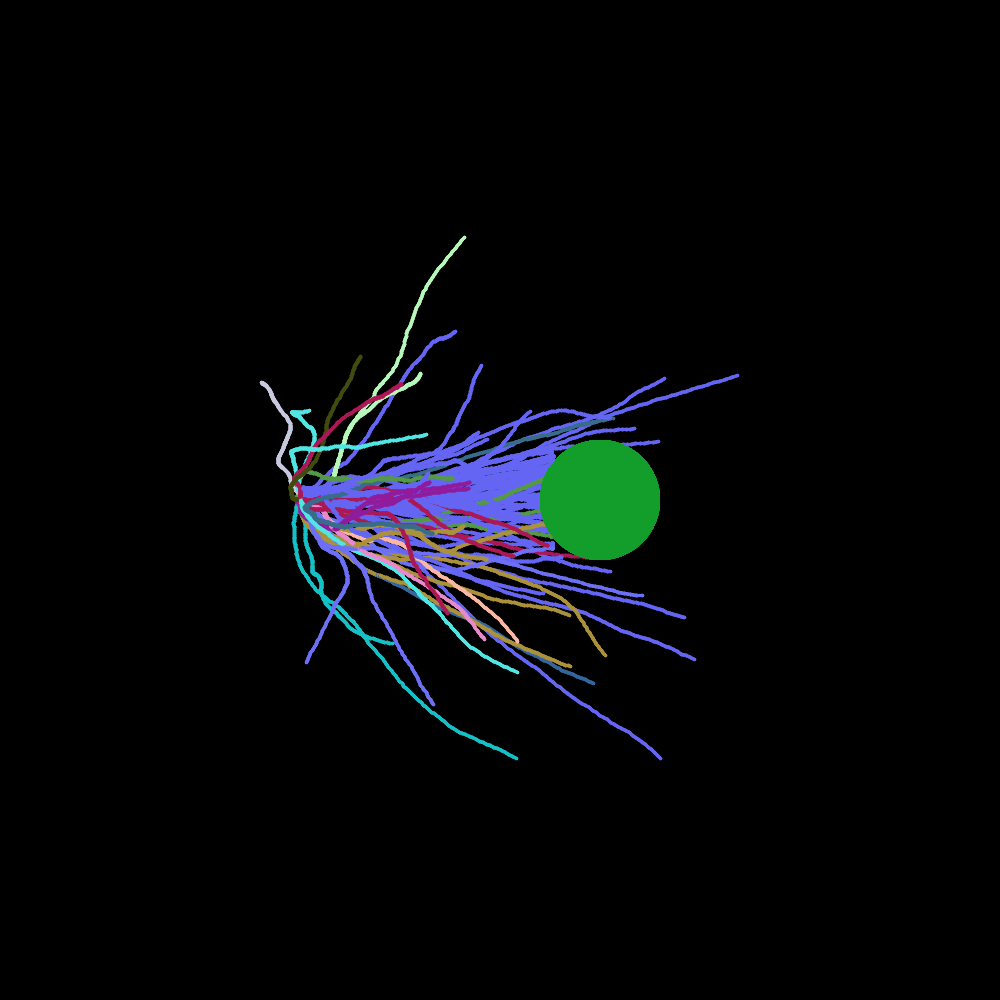
\includegraphics[width=\linewidth]{img/evoDefaultEnd.png}
				\caption[EvoDefaultEnd]{Evolution mit Defaultwerten nach 2100 Iterationen (eigene Darstellung)}
			\end{minipage}
		\end{figure} 
		\noindent Unten überströmen 300 Schnüre aus der linken oberen Ecke den Bildschirm, es sollten mindestens 75 Schnüre die Zielscheibe treffen. Nach 1800 Iterationen haben schon mindestens die Hälfte der angestrebten 75 Schnüre getroffen.\\
		Bildgenerierung:,,Menübar/Beispiele/SHopf/Evolution/EvoEcke''\\
		\begin{figure}[H]
			\centering
			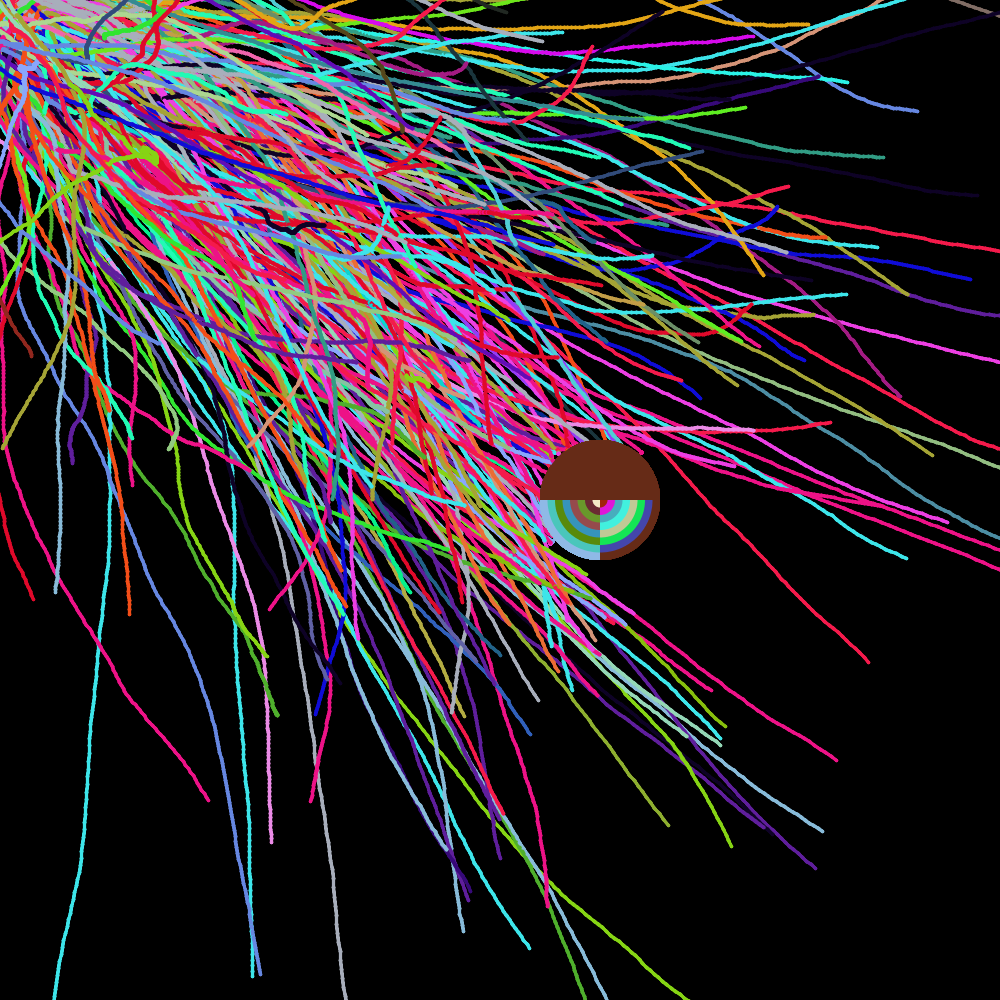
\includegraphics[width=0.5\linewidth]{img/evoEcke.png}
			\caption[EvoEcke]{Evolution mit 300 Schnüren nach 1800 Iterationen (eigene Darstellung)}
		\end{figure} 
		\noindent Unten nun eine Abbildung von nur 32 Schnüren, die alle die Zielscheibe treffen sollen. Hier muss man sehr viel Geduld aufbringen, falls man das vollständige Ergebnis sehen möchte, sofern dies überhaupt geschieht. Hier haben nach 6279 Iterationen noch nicht einmal die Hälfte der Schnüre getroffen. Die Farben haben sich aber schon angeglichen.\\
		Bildgenerierung:,,Menübar/Beispiele/SHopf/Evolution/EvoWenig''\\
		\begin{figure}[H]
			\centering
			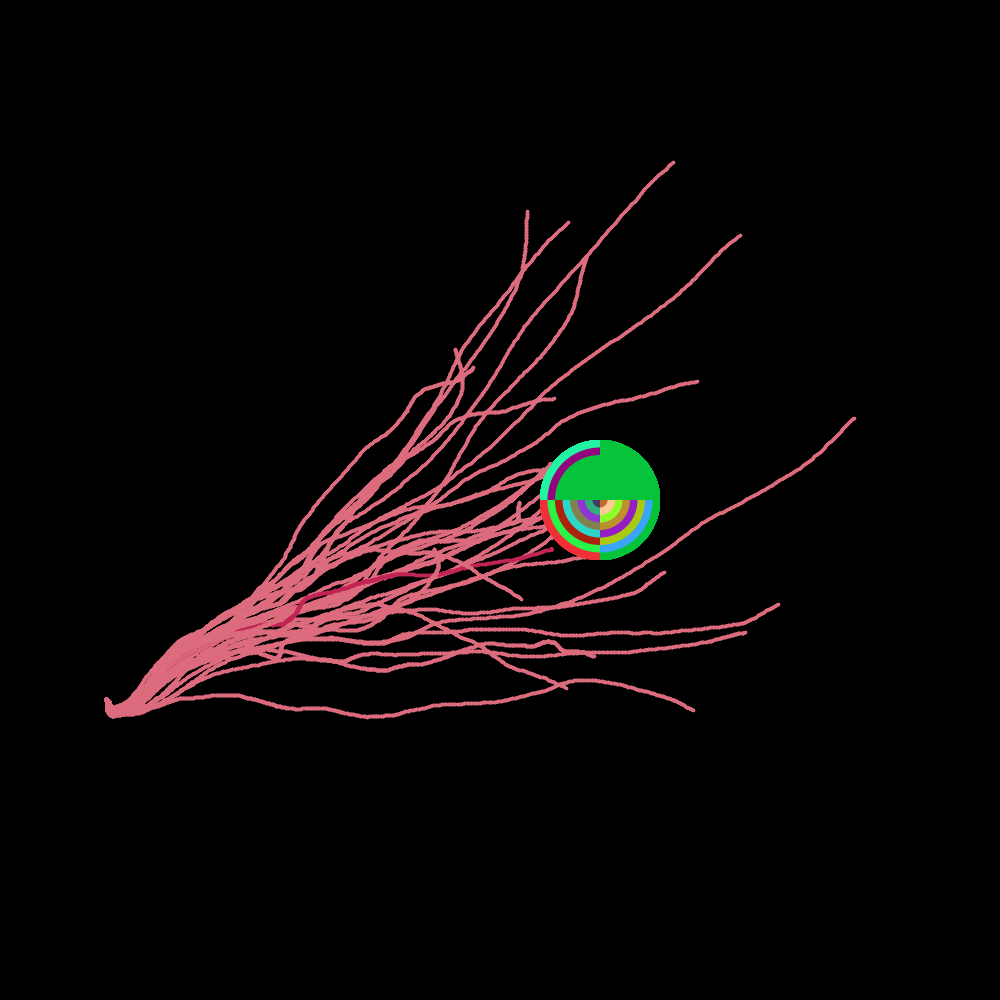
\includegraphics[width=0.5\linewidth]{img/evoWenig.png}
			\caption[EvoWenig]{Evolution mit 32 Schnüren nach 6279 Iterationen (eigene Darstellung)}
		\end{figure} 
				
		\paragraph{Stärken und Schwächen}$~$\\
		Die Stärken liegen hier vor allem in der selbstlernenden Art des Algorithmus. Wenn der Algorithmus mit echten Zufallszahlen läuft und man ein bestimmtes Ziel für ein Bild vor Augen hat, könnte man sich diesem auf immer neue Weise annähern und immer andersartige Kreationen erschaffen. Mit ein paar Modifizierungen könnte man hier auch den Benutzer mit einbinden, so dass er interaktiv an der Gestaltung von Bildern einwirken könnte.
		Die Schwächen liegen allerdings in der langen Laufzeit. Ein Bild ist nicht nach einer Lebensspanne der Objekte fertig, sondern braucht mehrere Generationen. Hier liegt es an dem Benutzer, wie viel Geduld er aufbringt.\\
		Der Algorithmus ist für die Kooperation und für die Einzelgenerierung geeignet, da er gut für sich allein wirkt, aber auch mit anderen Generatoren ein sehr schönes Ergebnis liefert. Hier können die anderen Generatoren dafür sorgen, dass das Ziel sich z. B. im L-System Baum befindet und die Schnüre auf diesen zusteuern usw.\\
		
	\subsubsection{Kooperation der eigenen Generatoren}
		Hier nun drei Beispiele, wie die eigenen Generatoren zusammenwirken können:\\
		Unten kooperieren ein L-System, ein Schwarm und ein weiteres L-System zusammen. Der rechte von den untersten Bäumen beeinflusst hier das Hindernis, dass der Schwarm meiden soll. Dies sieht man sehr schön an der freien Fläche rund um den Wipfel des Baumes.
		Außerdem werden von den Bäumen die Farbe und die Startinitialisierung der Boids beeinflusst. Der Schwarm seinerseits beeinflusst durch seine Einstellungen die Alphawerte der anderen Bäume und dass diese entartet sind.\\
		Bildgenerierung:,,Menübar/Beispiele/SHopf/Kooperation/Unterwasserwelt''\\
		\begin{figure}[H]
			\centering
			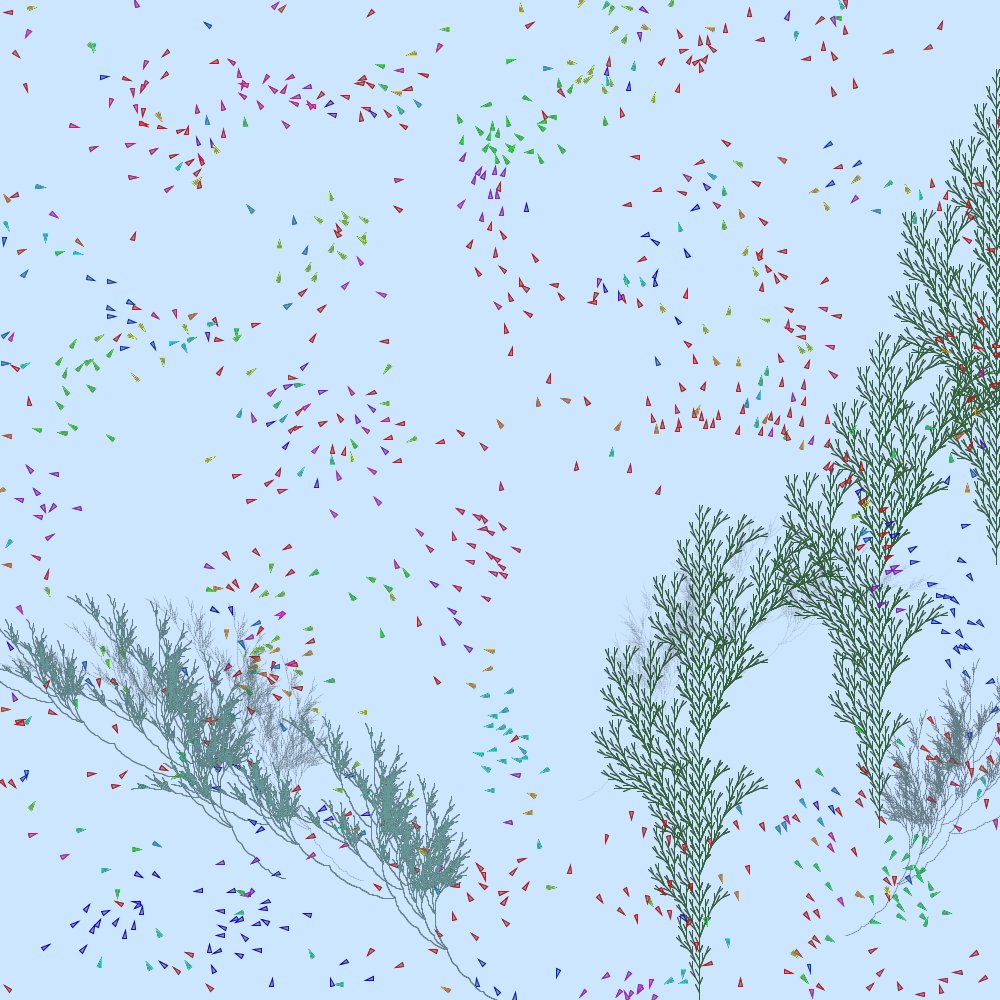
\includegraphics[width=\linewidth]{img/unterwasserwelt.png}
			\caption[Unterwasserwelt]{Kooperation L-System, Schwarm, L-System (eigene Darstellung)}
		\end{figure} 
		\noindent Unten kooperieren ein L-System, Evolution und ein weiteres L-System zusammen. Die oberen Bäume beeinflussen hier das Ziel der Evolutionsschnüre, welches sich wie man sieht in einem Baumwipfel befindet. Auch werden Farbe und Startinitialisierung der Schnüre von den Bäumen manipuliert. Die Evolution beeinflusst seinerseits den blauen Baum. Dieser wird dadurch in die andere Richtung gezeichnet.\\
		\begin{figure}[H]
			\centering
			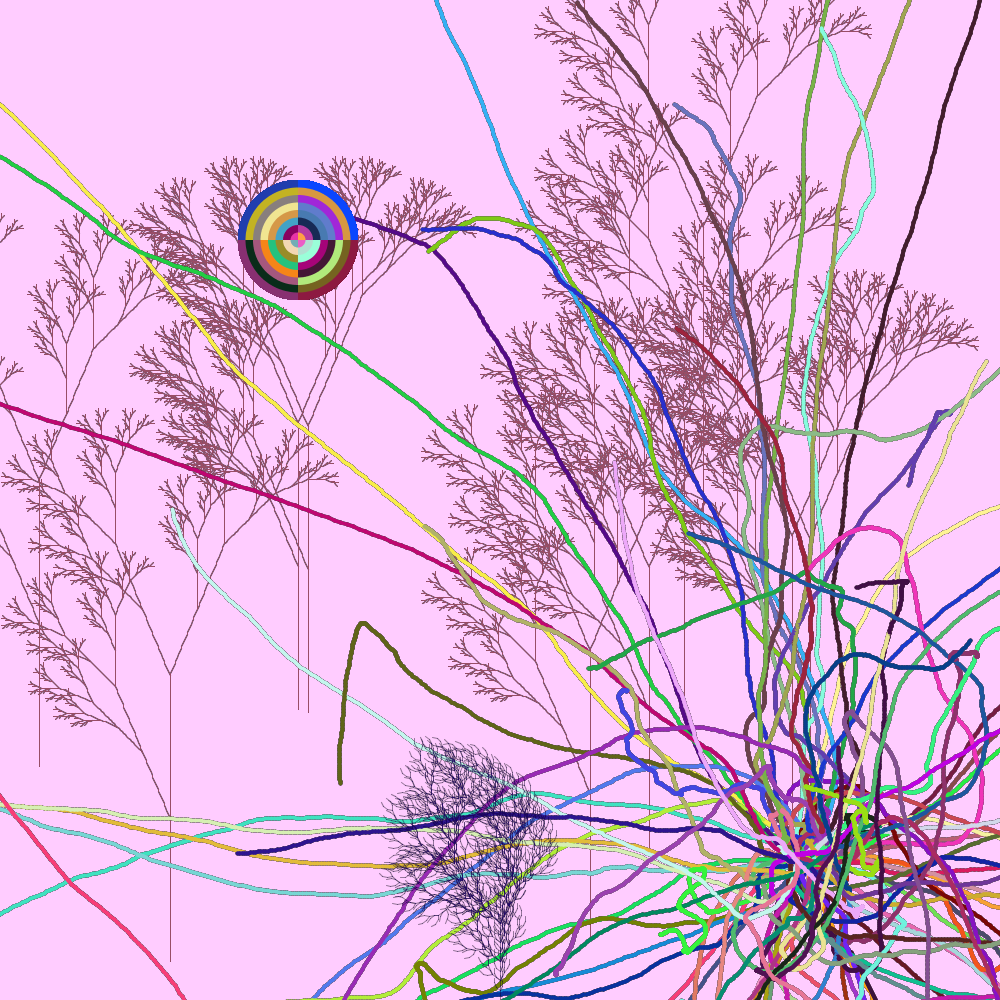
\includegraphics[width=\linewidth]{img/dschungel.png}
			\caption[Dschungel]{Kooperation L-System, Evolution, L-System (eigene Darstellung)}
		\end{figure} 
		\noindent Unten kooperieren ein Schwarm, Evolution und ein L-System zusammen. Der Schwarm zieht mit ausgeschaltetem Verlauf als Dreiecke seine Bahnen und beeinflusst das Ziel der Evolution. Die Startposition der Schnüre lenken ihrerseits die Ausrichtung der Bäume. Auch die Farben und Startinitialisierungen der Schnüre und die Größe der Bäume werden durch die Parameter der vorherigen Generatoren manipuliert.\\
	 	\begin{figure}[H]
	 		\centering
	 		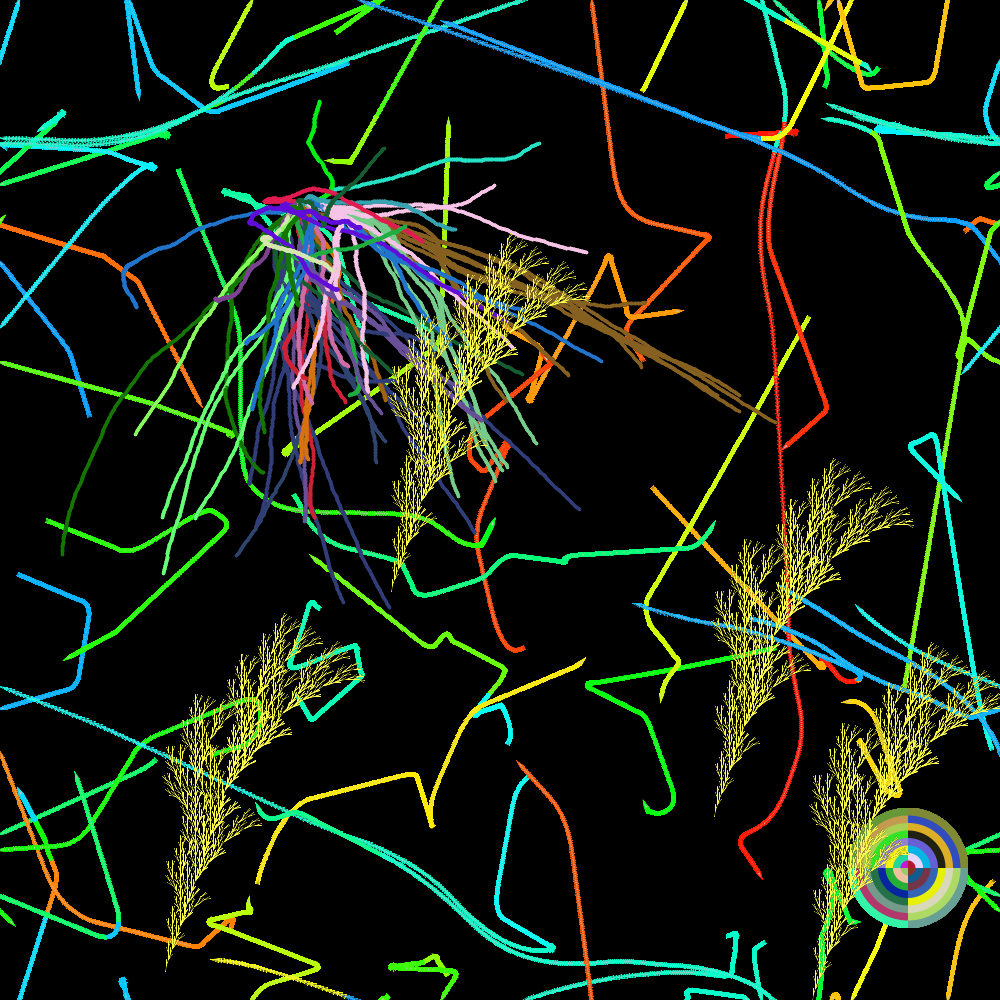
\includegraphics[width=\linewidth]{img/feuerwerk.png}
	 		\caption[Feuerwerk]{Kooperation Schwarm, Evolution, L-System (eigene Darstellung)}
	 	\end{figure} 
\end{document}
			\subfile{shopf/shopf}
			\clearpage
		\subsection{Generatoren von Gino Rißland}
			\subfile{gino/new_Ausarbeitung_mit_Gino}
			\clearpage
		\subsection{Generatoren von Bastian Winzen}
			% \documentclass[../mciAusarbeitung.tex]{subfiles}

\usepackage[utf8]{inputenc}
\usepackage[T1]{fontenc}
\usepackage{lmodern}
\usepackage[german]{babel}
\usepackage[fixlanguage]{babelbib}
\selectbiblanguage{german}
\usepackage{amssymb}
\usepackage{graphicx}
\usepackage{url}
\usepackage{float}
\usepackage{wrapfig}

\title{Fachpraktikum MCI (01513) - WS 2021/22}
\author{Gruppe 2\\
	Bastian Winzen}
\date{\today}

\begin{document}
Im Folgenden werden drei im Fachpraktikum entwickelte Implementationen von Bildgeneratoren vorgestellt. Die Ausarbeitungen basieren auf einem Algorithmus zur Schwarm Simulation, der Berechnung und Darstellung von Lindenmayer-Systemen (L-Systeme) oder befolgen Evolutionsprinzipien zur Erstellung eines Bildes.


\subsubsection{BWinzen::Schwarm - Schwarm Simulation}
	Die Entwicklung einer Schwarm Simulation erfolgte nach dem Vorbild der Flocking Simulation von Craig W. Reynolds aus dem Jahre 1986 \cite{reynolds1987flocks}.
	Kern dieses Ansatzes ist es, dass jedes Element im Schwarm sich selbst organisieren und ausrichten kann. Jedes dieser Elemente kennt seine Position, seine aktuelle Geschwindigkeit und kann auch diese Werte von allen anderen Elementen im Schwarm erfassen. Reynolds bezeichnet diese Elemente als ``Boids'', eine Wortneuschöpfung aus Bird und Android, die eine künstliche Simulation von Vogelverhalten andeutet.\\
	
	Um als ein Schwarm wahrgenommen zu werden müssen viele einzelne Komponenten in der Wahrnehmung zu einer Einheit bzw. Gruppe verschmelzen. Folgende Kriterien unterstützen diese Einordung: 1. \textit{Prinzipien der Wahrnehmung}: Gruppierung durch Form und Größe/Minimierung des Popup Effektes. Die Elemente weisen eine ähnliche Form und Größe auf. 2. \textit {Phänomene der Wahrnehmung}: ``gemeinsames Schicksal''. Geringe Entfernung, gleiche Geschwindigkeit und Ausrichtung implizieren eine Einheit. \cite{PetersSS21EMCI}.\\
	
	Um das Verhalten eines Schwarms zu simulieren, werden von Reynolds drei Grundkräfte genannt, die auf die Boids einwirken. Diese errechnen sich individuell für alle Elemente aus den Positionen und Geschwindigkeiten aller anderen Elemente im Schwarm.
	\begin{itemize}
	\item[]Die erste genannte Kraft ist die \textbf{``Collision Avoidance''} - zu Deutsch \textbf{Separationskraft}. Diese soll eine Kollision zwischen zwei Boids verhindern. Je näher sich zwei Elemente sind, desto stärker wird ihr Bestreben sich von einander zu entfernen.
	\item[]Die zweite genannte Kraft ist das \textbf{``Velocity Matching''} - zu Deutsch \textbf{Ausrichtungskraft}. Diese soll Boids so ausrichten, dass sich ihre Bewegungsvektoren immer mehr angleichen.  
	\item[]Die dritte genannte Kraft ist das \textbf{``Flock Centering''} - zu Deutsch \textbf{Kohäsionskraft}. Sie ist die Gegenkraft zur Separation und verhindernd ein zu starkes Auseinanderdriften der Boids. Der Kraftvektor zeigt auf den errechneten Mittelpunkt aller Elemente und bezeichnet die Intention aller Elemente sich an einem einzelnen Punkt im System zu versammeln.
	\end{itemize}
	
	Je nach Zusammenspiel dieser 3 Kräfte ergibt sich ein unterschiedliches Bild. Für die Implementation im Rahmen dieses Praktikums wird jede Kraft vom Anwender mit einem Faktor konfiguriert. So kann der Nutzer bestimmen ob er gleichmäßig verteilte Boids oder Boids, die sich in wenigen Punkten sammeln sehen möchte.\\
	In welchem Radius die Boids für die Berechnung der drei Grundkräfte herangezogen werden ist einzeln für jede Kraft konfigurierbar.\\\\
	Das berechnen der Kräfte für jedes Element im Schwarm hat eine Laufzeit von $O(n^2)$ wobei n der Anzahl aller Elementen entspricht. Für die Berechnung eines Elements muss immer jedes andere Element herangezogen werden.
	Die Konfiguration des Radius schränkt die Auswahl der Elemente, welche in die Berechnung der Kräfte einfließen jedoch ein. Um die Elemente im Radius zu ermitteln müssen dennoch zunächst alle Boids betrachtet werden.
\begin{wrapfigure}{r}{0.5\linewidth}
	\center
	\includegraphics[width=8cm]{"img/quadtree.png"}
	\caption{Beispiel eines Quadtrees entnommen aus \cite{DavidEppstein2005}}  
\end{wrapfigure}	
	Dieses Laufzeitverhalten stellt ein Problem dar, wenn die Anwendung auch mit vielen Boids flüssig laufen soll. \\
	Um meine hohe Anzahl Boids in der Anwendung zu ermöglichen wurde ein Quadtree implementiert und für die Datenhaltung der Boids verwendet. Dieser ermöglicht das Prinzip ``Divide and Conquer'' im zweidimensionalen Raum. Zusammengefasst kann der der Quadtree wie folgt beschrieben werden: \\
	Jedes Baumverzeichnis hat feste geometrische Grenzen. Zudem kann jedes Baumverzeichnis nur eine maximale Anzahl an Objekten beinhalten. Wird die maximale Anzahl überschritten wird der Bereich in 4 Teilbereiche unterteilt für die jeweils ein Baumverzeichnis instanziiert wird. Die Objekte werden nach ihrer räumlichen Anordnung in die entsprechenden Unterverzeichnisse einsortiert.\\	
	Durch die Nutzung des Quadtrees können Elemente mit einer Laufzeit von Durchschnittlich $O(ln(n))$ anhand ihrer Position gefunden werden bzw. alle Elemente in einem Radius gequeryt werden. Die Laufzeit pro Iteration beläuft sich auf $O(n*ln(n))$ \cite{Samet}.\\
	Um die Performance des Schwarms zu verbessern wurde die Berechnung vom Zeichenvorgang abgekoppelt. Boids haben 2 Zustände, den aktuellen Zustand sowie den Zustand für die nächste Iteration. In jeder Iteration wird der neue Zustand errechnet. Dies geschieht multithreaded und zur Berechnung werden die aktuellen Status der anderen Boids verwendet. Sind alle neuen Zustände berechnet werden sie als aktuell gesetzt und die Boids werden gezeichnet. Da die Renderer Statemachines sind, muss das Zeichnen synchron ablaufen.\\
	Bei den Schnittstellendefinitionen der Boids wurde darauf geachtet, dass zusätzlich zu den drei Grundkräften eine weitere Kraft in die Berechnung des neuen Zustands einfließen kann. Ein Beispiel für eine solche Kraft ist die Anziehung oder Abstoßung eines im Kooperation Kontext definierten Punktes.\\
	Ein weiteres Feature der Implementierung ist die Farbdiffusion. Mit entsprechenden Einstellungen wird die Farbe der Boids in jeder Iteration neu berechnet. Dafür werden die Farben der Boids im kleinsten der gewählten Radius zusammengerechnet und ein Durchschnittswert errechnet. Dieser Farbwert wird als neuer Farbwert des Boids gesetzt. Zudem gibt es eine spezielle Möglichkeit der Kooperation, bei der die Boids die Farbe des Pixels der aktuellen Position aus der vorangegangenen Iteration übernehmen. Dafür muss in den Parametern ein entsprechender Filter definiert werden, der definiert welche Farbwerte übernommen werden.
	
\paragraph{Parameter-Beschreibungen für BWinzen::Schwarm}
\begin{itemize}
	\setlength\itemsep{-0.1em}
	\item\textit{Anzahl:} Anzahl der Boids in der Simulation
	\item\textit{Ausrichtung:} Faktor für die Gewichtung der Ausrichtung
	\item\textit{Kohäsion:} Faktor für die Gewichtung der Kohäsion 
	\item\textit{Separation:} Faktor für die Gewichtung der Separation 
	\item\textit{Radius Aus.:} Radius für die Betrachtung anderer Boids zur Berechnung der Ausrichtung
	\item\textit{Radius Sep.:} Radius für die Betrachtung anderer Boids zur Berechnung der Separation
	\item\textit{Radius Kohäsion:} Radius für die Betrachtung anderer Boids zur Berechnung der Kohäsion
	\item\textit{Form:} Form der Boids. Derzeitige Varianten: {Kreise, Linien, Pole, Rechtecke, Quadrate, Dreiecke, Zufällige Formen}
	\item\textit{Größe:} Größe der Boids
	\item\textit{Feste Größe:} Aktiviert - Alle Elemente die gewählte Größe, Deaktiviert - Größe zufällig und maximal Wert begrenzt
	\item\textit{Anfangsfarbe:} Grundlage zur Berechnung der Elementfarbe 
	\item\textit{Farbmodus:} siehe \ref{parametrisierung} Allgemeine Parametrisierung>>Farbmodus
	\item\textit{Farbverläufe:} Aktiviert -  Alle Boids aus dem kleinsten Radius der drei gewählten Radius werden zur Berechnung der nächsten Farbe herangezogen. Für jeden Farbkanal wird der Durchschnittswert aller Boids im Radius errechnet und als neue Farbe gesetzt.
	\item\textit{CoopModus Farbenübernahme:} Das aktuelle Pixel des bestehenden Bildes wird pro Iteration über Filter geprüft. Wenn der bestehende Farbwert dem ausgewählten Filter genügt, wird der Farbwert übernommen. Aktuelle stehen folgende Filter zur Verfügung:
		\begin{itemize}
		\setlength\itemsep{-0.1em}
			\item Keine Übernahme,
			\item Hohe Farbkanal Werte (> 0xF8),
			\item Mittel Starke Farbkanal Werte (> 0xC4),
			\item Schwache Farbkanal Werte (> 0x80),
			\item Starker Rot Wert (> 0xF8),
			\item Starker Grün Wert (> 0xF8),
			\item Starker Blau Wert (> 0xF8),
			\item Starker Blau Wert (> 0xF8), Helle (Brightness > 0.7),
			\item Dunkle (Brightness < 0.3),
			\item Hohe Sättigung (Saturation > 0.7)
		\end{itemize}
	\item\textit{KoopModus Orientierung:}  siehe \ref{parametrisierung} Allgemeine Parametrisierung>>KoopModus Orientierung
	\item\textit{Max. Geschwindigkeit:} Maximale Geschwindigkeit der Boids.
	\item\textit{Max. Beschleunigung:} Maximale Beschleunigung der Boids. Je höher der Wert, desto abrupter sind die Richtungswechsel.
	\item\textit{Einheitliche Geschwindigkeit:} Aktiviert - Alle Boids die gleiche Geschwindigkeit. Diese Option hat sehr großes Einfluss auf das Verhalten des Schwarms.
	\item\textit{Kanten Verhalten:}
		\begin{itemize}
		\setlength\itemsep{-0.1em}
			\item\textit{Konzentrisch:} Verlassen die Boids das Fenster, werden sie auf die Gegenseite versetzt. Dabei wird die Richtung beibehalten.
			\item\textit{Spiegeln:} Verlassen die Boids das Fenster, wird ihr Geschwindigkeitsvektor an der Kante die überschritten wurde, gespiegelt.
			\item\textit{Rotation:} Sind die Boids dabei das Fenster zu verlassen, werden sie abgeleitet/rotiert bis sie wieder in Richtung des Fensters fliegen. Je schneller sie fliegen um so stärker ist die Rotation ausgeprägt.
			\item\textit{Teleportation:} Verlassen die Boids das Fenster, werden sie an den Punkt des Kooperationskontextes teleportiert behalten aber ihren Richtungsvektor. Wenn die überschrittene Kante zu nah am Zielpunkt liegt wird der Richtungsvektor umgedreht.
		\end{itemize}	
	\item\textit{Farbenreservoirs nicht zeichnen:} Um Farben zur Übernahme in der Cooperation zu haben, wurden zu Testzwecken `Farbenreservoirs' gezeichnet. Zufällig wird ihre Farbe gesetzt und dabei darauf geachtet, dass die Farben übernommen werden können. Die `Farbenreservoirs'  sind Kreise die mit Gradienten gefüllt sind. Ihre Farbe und Bewegung wird durch den Seed zufällig bestimmt. Implementiert ist ein Rotation sowie ein alternierendes auseinanderdriften der Kreise. Diese beiden Eigenschaften können kombiniert werden, wodurch ein Spiralverlauf entsteht.
	\item\textit{Farben verblassen:} Diese Einstellung kommt nur zum Tragen wenn der Verlauf eingeschaltet ist. In jeder Iteration werden alle Pixel des Layers in ihrer Opacity um den eingestellten Wert verringert.
\end{itemize}	
%\pagebreak
\paragraph{Beispiele:}
Folgende Beispiele können im Konfigurator unter MenuBar>>Beispiele>>BWinzen>>Schwarm ausgewählt werden.

	\subparagraph{a)Batcave:} Dreiecke in einem Schwarm, die ihre Farbe an den Nachbarn anpassen und beim Überflug über Bildpunkte mit starken Farbkanalwerten (r oder g oder b über 0xF8) die Farbe des unterliegenden Pixels annehmen.	
	
	\subparagraph{b)2 Schwärme:} 2 Schwärme mit unterschiedlichem Randverhalten, Größe, Form und anderen Parametern.

	\subparagraph{c)Colorexplosion:} Ein Schwarm bestehend aus Linien. Die aktuelle wird mit der vorherigen Position des Boids durch eine Linie verbunden. Der Verlauf ist eingeschaltet und es wird in jeder Iteration der Alpha Wert des bestehenden Verlaufs um 10 reduziert.

	\begin{figure}[H]
		\begin{subfigure}{0.5\linewidth}
			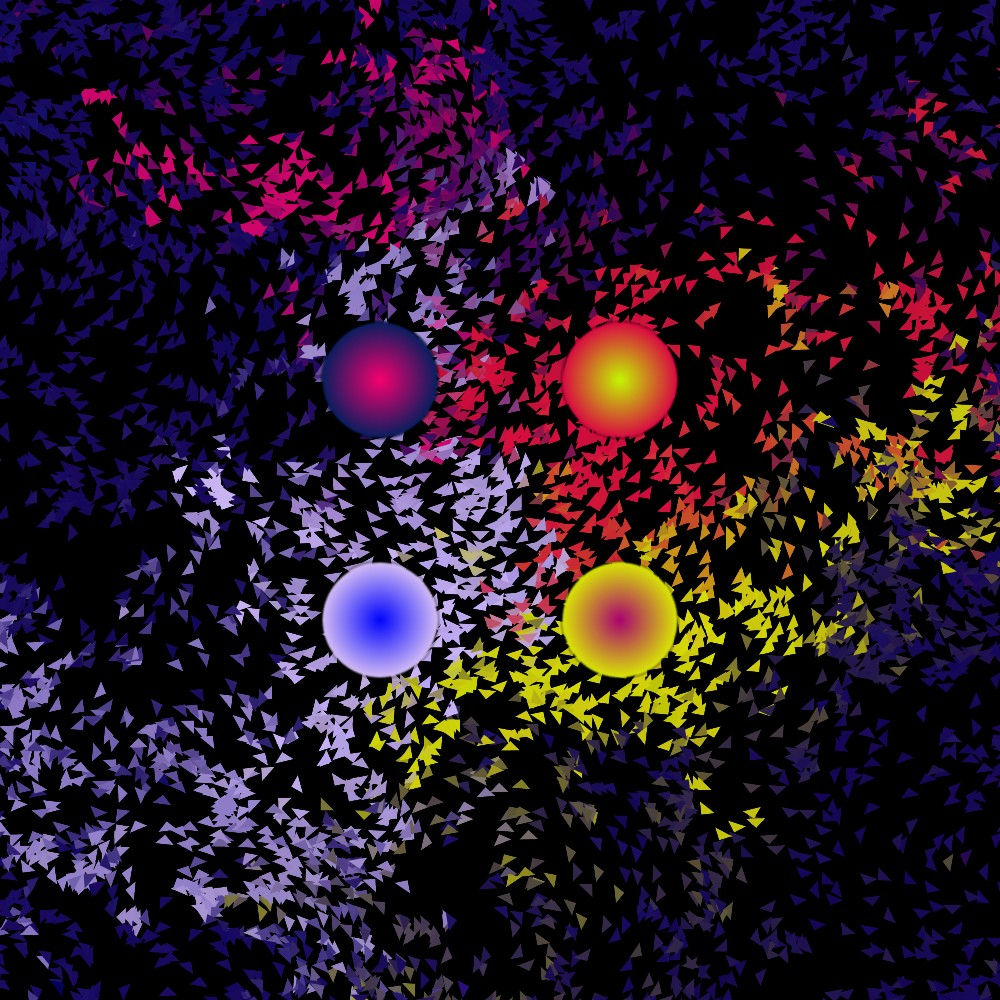
\includegraphics[width=0.95\linewidth]{"img/swarm_batcave.jpg"}
			\caption[Batcave]{\textbf{Batcave}}  
		\end{subfigure}	
		\begin{subfigure}{0.5\linewidth}
			
\includegraphics[width=0.95\linewidth]{"img/swarm_2x.jpg"}
			\caption[2 Schwärme]{\textbf{2 Schwärme}}  
		\end{subfigure}		
		\begin{subfigure}{0.5\linewidth}
	 		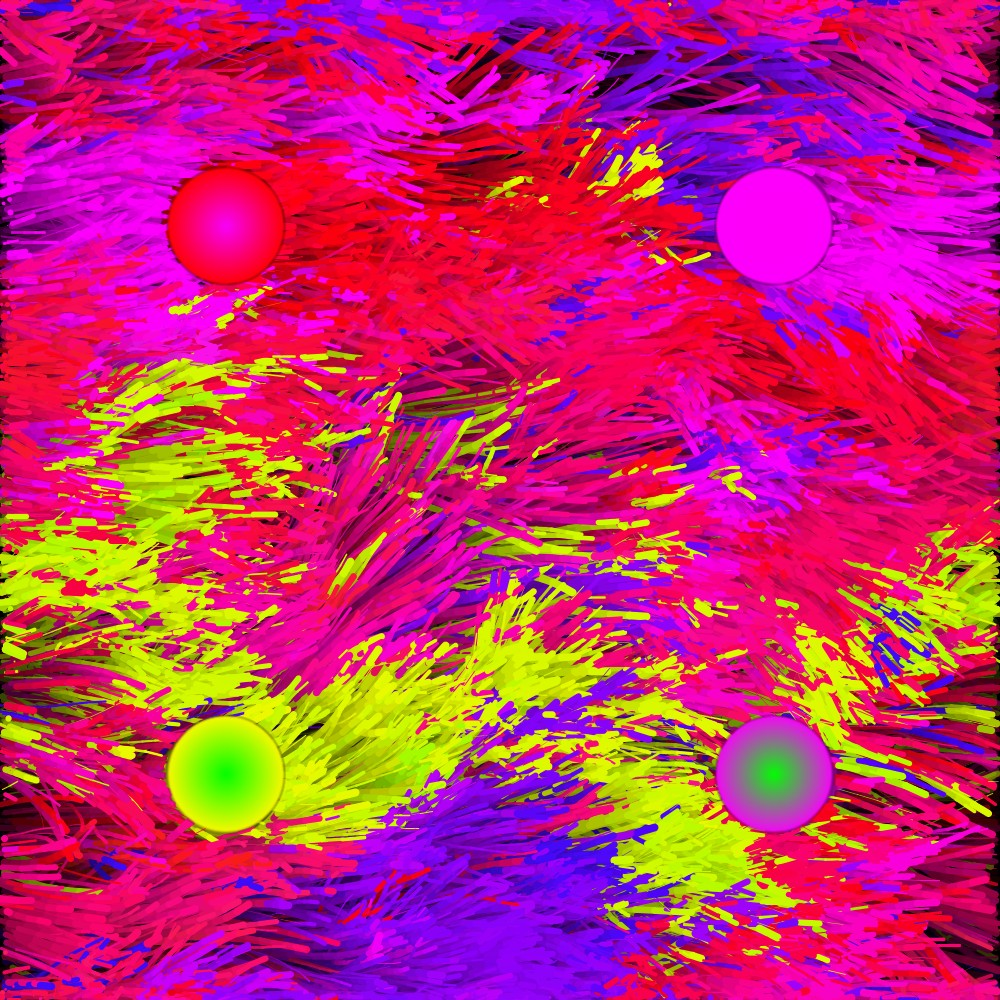
\includegraphics[width=0.95\linewidth]{"img/swarm_fading.jpg"}
			\caption[Colorexplosion]{\textbf{Colorexplosion}}  
		\end{subfigure}	
	\caption[BWinzen:Beispiele Schwarm]{BWinzen:Beispiele Schwarm}
\end{figure}

\subsubsection{BWinzen::LSystem \& BWinzen::LSystemBuilder - Berechnung und Darstellung eines L-System}
	Lindenmayer, ein Biologe aus der Mitte des 20. Jahrhundert, versuchte natürliche Strukturen wie Pflanzen und Bäume mathematisch zu beschreiben. Diese bei seinen Untersuchungen definierten mathematischen Gebilde nennt man heute `Lindenmayer-' bzw. `L-Systemen'.  
	
	Am Anfang eines L-Systems steht ein Alphabet im mathematischen Sinne. Ein Alphabet bezeichnet eine Menge von Zeichen. In einem L-System ist jedem Zeichen eine Visualisierungsregel zugeordnet.\\
	Das Axiom stellt die Startsequenz dar. Es ist eine Tupel beliebiger Elemente aus dem definierten Alphabets des L-Systems. Durch das Axiom wird das L-System initialisiert.\\
	Als Grammatik des L-Systems wird eine Menge von Ersetzungsregel bezeichnet. Diese definieren, welche Zeichen durch eine Reihe anderer Zeichen aus dem Alphabet ersetzet werden. Basiert jede Ersetzungsregel auf einem einzigen Zeichen, welches durch beliebig viele Zeichen ersetzt werden kann, handelt es sich um ein kontextfreies L-System. Gibt es Regeln, bei denen mehrere zusammenhängende Zeichen ersetzt werden, wird es als kontextsensitives L-System bezeichnet \cite{prusinkiewicz1990algorithmic}. Der im Rahmen dieser Arbeit implementierte Generator erzeugt kontextfreie L-Systeme.\\
	In jedem Iterationsschritt werden die Regeln der Grammatik auf die aktuelle Sequenz der Zeichen angewendet. So verändert sich die Sequenz in jedem Iterationsschritt.\\
	Ein Beispiel:
	\begin{itemize}
	\setlength\itemsep{-0.2em}
	\item[] Alphabet = {A,B,+,-}
	\item[] Axiom = A
	\item[] Regeln:
		\begin{itemize}
		\setlength\itemsep{-0.2em}
			\item[1.]A = AB
			\item[2.]B = +A-
		\end{itemize}
	\end{itemize}
	\begin{itemize}
	\setlength\itemsep{-0.2em}
		\item[] 0.Iteration Axiom = A 
		\item[] 1.Iteration AB \quad \quad \quad \quad \quad \quad \quad \quad \quad \quad \quad \quad \quad //Anwendung von Regel 1 
		\item[] 2.Iteration AB+A- \quad \quad \quad \quad \quad \quad \quad \quad \quad \quad \quad//Anwendung von Regel 1 und 2 
		\item[] 3.Iteration AB+A-+AB- \quad \quad \quad \quad \quad \quad \quad \quad //Anwendung von Regel 1 und 2 
		\item[] 4.Iteration AB+A-+AB-+AB+A--   \quad \quad \quad \quad  //Anwendung von Regel 1 und 2 
		\item[] 5.Iteration AB+A-+AB-+AB+A-+AB---   \quad  //Anwendung von Regel 1 und 2 
	\end{itemize}

	Bei der Visualisierung wird jedem Zeichen im Alphabet eine bestimmte Bedeutung zugetragen. So kann zum Beispiel `A' und `B' für vorwärts, `+' für eine rechts Drehung um 20\textdegree\:sowie `-' für eine Linksdrehung um 20\textdegree\:stehen. Wenn man nun die Zeichenkette und die damit Verbunden Zeichenanwendungen mit einem virtuellen Stift nachzeichnet entsteht ein Bild. \\
	Eine Erweiterung der Möglichkeiten eines L-Systems entsteht durch den Einsatz eines FIFO-Speichers. Ein Beispielhafte Belegung von Zeichen wäre:\\
	 Bei dem Zeichen `$[$' wird die aktuellen Position gesichert bei der zugehörigen `$]$' Klammer wird die aktuelle Position wieder geladen.\\
	 So können beispielsweise Verästelung entstehen. Iterationsbedingte Faktoren die Längen und Winkel ändern, ermöglichen eine große Anzahl an zusätzlich darstellbaren Formen.\\
	 Ersatzregeln können auch bedingt formuliert werden, sodass sie nur unter bestimmten Voraussetzungen angewendet werden. Im Zuge des Praktikums wurde auf diesen letzten Schritt der Erweiterung verzichtet und anstelle dessen die Mehrfachbelegung von Variablen in den Ersetzungsregeln erlaubt. Wenn 2 Regeln auf derselben Variable anwendbar sind, entscheidet der Zufall welche von ihnen Verwendung findet. Das in der Konfiguration auswählbare L-System `geordnetes Chaos' benutzt dieses Prinzip um wahlweise eine Ellipse zu zeichnen oder den Baum weiter fortzusetzen.\\
Die `LSystem' Klasse spiegelt das L-System in einem Iterationsschritt dar. Sie enthält das Alphabet (ein Set aus `AlphabetLetter's), die aktuelle Sequenz, sowie alle Ersetzungsregeln. Mit \textit{LSystem nextIteration()} kann das L-System der nächsten Iteration errechnet und instantiiert werden.\\
Die `LSystemTree' Klasse ist für die Visualisierung des L-Systems zuständig. Die erste rekursive Implementation der Visualisierung resultierte in sehr schlechter Performance. Um diesem Problem entgegenzuwirken wurde die Errechnung der Zeichen von dem eigentlichem Zeichenvorgang abgekoppelt. So kann die Zeichenanweisung in mehreren Threads vorberechnet werden und zudem für den mehrmaligen Gebrauch im Cache gespeichert werden.
 Performance und User-Experience mit dem L-System-Generator konnten durch diese Änderung im Algorithmus massiv verbessert werden. Im Rahmen dieser Anpassung wurde die `LSystemTree' Klasse abstract und eine rekursive sowie eine nicht rekursive Variante für die Benutzung vorbereitet. Beide Varianten brauchen unterschiedliche Visualiserungsregeln bzw. Berechnungsregeln. Aktuell sind fast alle auswählbaren L-Systeme auf die nicht rekursive Variante migriert.\\
	Die Benutzung von Farbgradienten bei der Darstellung ist durch die Umstellung auf einen nicht rekursiven Algorithmus leicht möglich. Jede Linie kennt nun die eigene relative Position zum Ausgangspunkt. Die Darstellung fängt immer im Punkt 0,0 an wird anschließend rotiert und verschoben. So wird die Farbe nach Abstand zum Ausgangspunkt errechnet. Das Beispiel `Sierpinski Dreiecke' verdeutlicht dies.

\paragraph{Beschreibung der Parameter für BWinzen::LSystem:}
	Der L-System Generator kann durch 2 Schnittstellen konfiguriert werden. Diese Unterscheidung wurde gewählt, da der Aufwand ein L-System mit Regeln und Axiom einzugeben sehr hoch ist. Durch diese Implementation kann entweder auf vordefinierte L-Systeme zurückgegriffen oder die Parameter manuell konfiguriert werden. Eine Zusammenfassung in einem einzigen Abschnitt der GUI war aufgrund des generischen Aufbaus des Generator-Konfigurationsbereiches nicht möglich. Die Form einer zweiten Eingabemaske macht ein Konfiguration möglich, ohne auf speziell für diesen Zweck entwickelte GUI-Elemente zurückgreifen zu müssen.\\
	Für den `LSystemBuilder' sind folgende Zeichen des Alphabets schon vorbelegt.\\
	Bei `$[$' wird die aktuellen Position gesichert und bei der zugehörigen `$]$' Klammer wird die aktuelle Position wieder geladen.\\
	\indent + ist eine Rechtsdrehung.\\
	\indent - ist eine Linksdrehung.\\
	\begin{itemize}
	\setlength\itemsep{-0.1em}
		\item\textit{Axiom:} (Nur BWinzen::LSystemBuilder)Definieren eines Axioms
		\item\textit{Rule0-5:} (Nur BWinzen::LSystemBuilder)Definieren der Regeln der Grammatik
		\item\textit{Winkel:} (Nur BWinzen::LSystemBuilder) Winkel für eine Rechtsdreheung bei + und eine Linksdrehung bei - 
		\item\textit{LSystem:} (Nur BWinzen::LSystem)Wählen eines vordefinierten LSystems
		\item\textit{Anzahl:} Die Anzahl der LSysteme die vom Generator dargestellt werden sollen.
		\item\textit{Größe:} Die Größe des LSystems.
		\item\textit{gleiche Größe:} Aktiviert - alle erzeugten Darstellungen haben die gleiche Größe.  Deaktiviert - gewählte Größe stellt einen Maximalwert dar. Die eigentliche Größe wird durch eine (Pseudo)Zufallszahl bestimmt.
		\item\textit{Iterationen:} Anzahl der Iterationen, die dargestellt werden.
		\item\textit{Iterationsverzögerung:} Anzahl an Frames, die für einen Iterationsschritt gewartet wird.
		\item\textit{Strichfarbe:} Die Auswahl dient als Grundlage zur Berechnung der Farbe der Darstellungen. 
		\item\textit{Strichstärke:} Die Strichstärke der Darstellung.
		\item\textit{Farbmodus:} siehe \ref{parametrisierung} Allgemeine Parametrisierung>>Farbmodus
		\item\textit{Alpha Wert:} Setzt den Alpha Wert der Darstellungen. 
		\item\textit{KoopModus Orientierung:}  siehe \ref{parametrisierung} Allgemeine Parametrisierung>>KoopModus Orientierung
		\item\textit{Reihenfolge Umkehren:} Wenn die Option gewählt wurden ist, wird zu erst die höchste Iteration des L-Systems gezeichnet und danach die niedrigeren Iterationen. Bei vielen L-Systemen erlangt die Darstellung dadurch eine Art Tiefe wenn zwischen den Iterationen die Farbe variiert. 
		\item\textit{Rotation:} Wenn die Option gewählt wird startet die Darstellung des L-Systems mit einem zufälligen Anfangswinkel.
		\item\textit{XOffset/YOffset:} (Nur BWinzen::LSystemBuilder)Definiert einen X-/Y-Offset, der auf die zufällige Positionierung auf dem Bildschirm addiert wird. So kann das Wachstum der Darstellung Berücksichtigung finden. Ohne den Y-Offset würde eine Darstellung von Bäumen dazu führen das der unter Teil des Bildschirmes sehr leer wirkt. Da nur die dünnen Anfangs-`Stämme' gezeichnet werden.
	\end{itemize}
\paragraph{Beispiele:}
	Folgende Beispiele können im Konfigurator unter MenuBar>>Beispiel>>BWinzen>>LSystem ausgewählt werden.
		\subparagraph{a)Einfaches L-System:} Einfache Darstellung eines L-Systems in der 4.Iteration.\\
	\indent\indent Axiom = F\\
	\indent\indent Winkel = 30 \\
	\indent\indent Regeln: \\
	\indent\indent\indent 1. F = FF+[+F-F-F]-[-F+F+F] \\
	\indent\indent Zusatzregeln:\\
	\indent\indent\indent Die Länge der repräsentierenden Linie zu F wird in jeder Iteration halbiert.
	
	\subparagraph{b)Sierpinski Dreieck:} Dargestellt sind Sierpinski Dreiecke in der 6.Iteration. Die Farben sind zufällig und der Gebrauch von Farbgradient ist sichtbar.\\
	\indent\indent Axiom = F+G+G\\
	\indent\indent Winkel = 120 \\
	\indent\indent Regeln: \\
	\indent\indent\indent 1. G = GG \\
	\indent\indent\indent 2. F = F+G-F-G+F 
	\subparagraph{c)Milkyway:} Dargestellt sind Stern ähnliche L-Systeme in verschiedenen Größen, wie zum Beispiel Koch-Schneeflocken.
	\subparagraph{d)AutumnBlues:} Verschiedene Baum ähnliche L-Systeme in Herbstfarben.
	 
	
\begin{figure}[H]
	\begin{subfigure}{0.5\linewidth}
		
\includegraphics[width=0.95\linewidth]{"img/lsystem_simple.jpg"}
		\caption[Einfaches L-System]{\textbf{Einfaches L-System}}  
	\end{subfigure}
	\begin{subfigure}{0.5\linewidth}
		
\includegraphics[width=0.95\linewidth]{"img/lsystem_sierpinski.jpg"}
		\caption[Sierpinski Dreieck]{\textbf{Sierpinski Dreieck}}  
	\end{subfigure}		
	\begin{subfigure}{0.5\linewidth}
 		
\includegraphics[width=0.95\linewidth]{"img/lsystem_milkyway.jpg"}
		\caption[Milkyway]{\textbf{Milkyway}}  
	\end{subfigure}	
	\begin{subfigure}{0.5\linewidth}
 		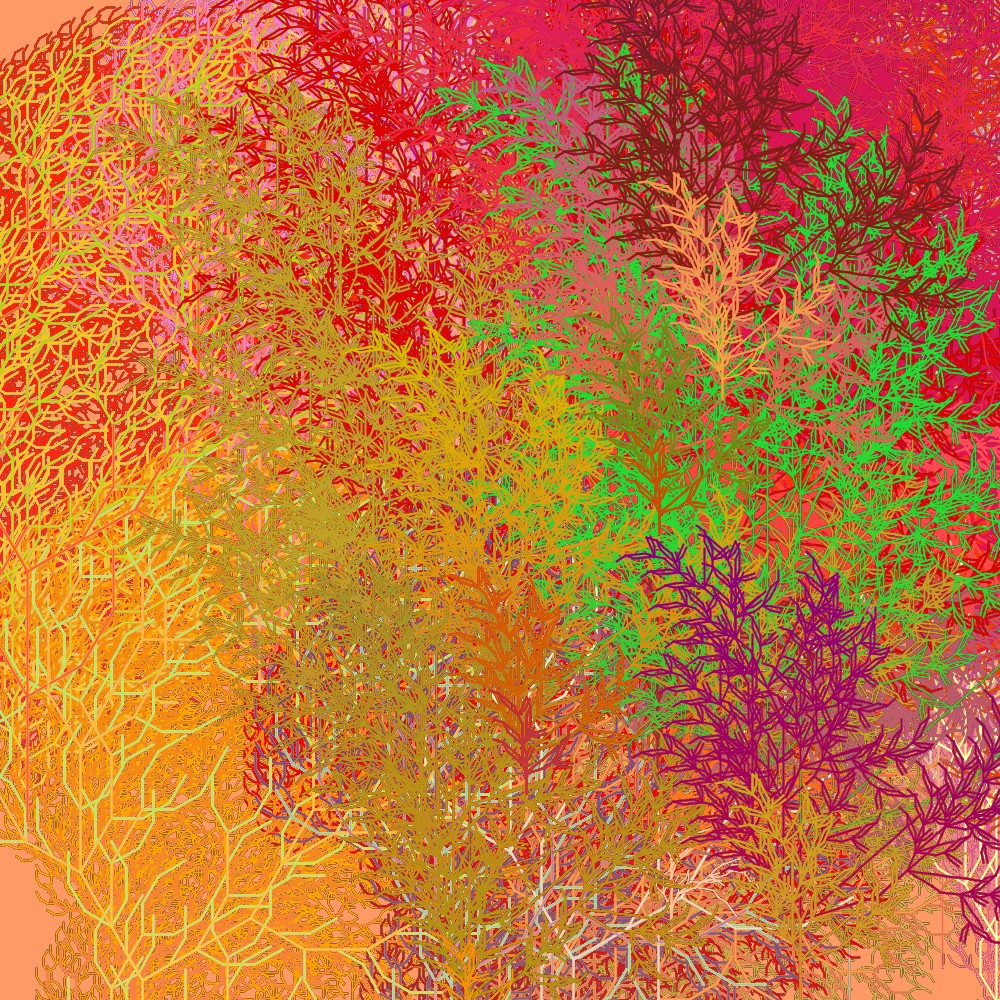
\includegraphics[width=0.95\linewidth]{"img/lsystem_autumn.jpg"}
		\caption[AutumnBlues]{\textbf{AutumnBlues}}  
	\end{subfigure}	
	\caption[BWinzen:Beispiele L-System]{Beispiele L-System}
\end{figure}

	
\subsubsection{BWinzen::3DImageEvolution - Evolutionsprinzipien}
		Im Jahr 1859 veröffentlichte Charles Darwin sein Buch ``On the Origin of Species''. Dieses stellt aus heutiger Sicht einen der größten Meilensteine der Biologie dar. Das Prinzip ``Survival of the fittest'' umschreibt die Tatsache, dass die Entwicklung von Lebewesen nicht gezielt abspielt. Vielmehr werden Individuen aussortiert, welche nicht an die natürlichen Umgebungsfaktoren angepasst sind. Nur wer an die Gegebenheiten angepasst ist, kann bestehen und sich fortpflanzen. Da die Nachkommen ihren Vorfahren physiologisch ähnlich sind haben diese wiederum eine bessere Chance zu überleben und bestimmte Eigenschaften bilden sich so in der Gesamtpopulation heraus. Dieses Prinzip ist heute als Evolutionsprinzip bekannt und hat seinen Weg in viele andere wissenschaftliche Disziplinen gefunden, insbesondere auch in die Informatik. \\
		Heutige Computersysteme rechnen sehr schnell und viele Dinge der Wirklichkeit können durch Modelle mit all ihren Eigenschaften abgebildet werden. So können in wenig Zeit viele Varianten einer Thematik simuliert werden. Dies kann als Basis für einen evolutionäre Entwicklung eines Computermodells genutzt werden.\\
		Bei nicht deterministischen Problemen, kann das Prinzip der Evolution ein passender Ansatz sein um zu einer guten Lösung zu kommen. Wie geeignet die aktuelle Variante des Computermodells in einer Simulation ist, wird durch eine Fitnessfunktion bestimmt. Der Wert der Fitnessfunktion bestimmt die Güte der Simulation und stellt das Gegenstück zur Überlebens- / Fortpflanzungswahrscheinlichkeit in der klassischen Evolution dar.
		 Liefert die Fitnessfunktion einen guten Wert wird die Simulation leicht abgewandelt und überprüft ob noch bessere Werte erreicht werden können. Ist der Wert der Fitnessfunktion schlecht wird der aktuelle Evolutionszweig verworfen.
		
		Der Generator BWinzen::3DImageEvolution besteht aus einem sogenannten Shooter und einer virtuellen Leinwand. Die Leinwand ist auf der Z-Achse versetzt, im Raum platziert. Während der Animation schießt der Shooter Objekte in die Richtung der Leinwand. Eine zweidimensionale Perlin-Noise Funktion hilft dabei die Bewegungen des Shooters flüssig aber zufällig aussehen zu lassen. 
		Wenn die verschossenen Objekte die Leinwand treffen gibt es 2 Möglichkeiten. Wird die Fitness des getroffenen Pixels auf der Leinwand nicht verbessert fliegt das Objekt durch sie hindurch. Wird jedoch die Fitness des getroffenen Pixels verbessert bleibt das Objekt auf der Leinwand haften. Je nachdem wie gut der neue Fitnesswert ist, werden Referenzen (je besser desto mehr) auf den aktuellen Schusses in eine priorisierte Queue abgelegt. Die Queue ist von der Größe begrenzt und hält nur Referenzen mit den besten Fitnesswerten. Die Referenzen enthalten die Farben der verschossenen Objekte als auch die Zielkoordinate.\\
		Zu jedem Zeitpunkt können maximal eine eingestellte Anzahl an Elementen in der Animation umherfliegen. Verlässt ein Element den sichtbaren Bereich bzw. ist zu weit auf der Z Achse fortgeschritten, wird es vom Shooter erneut verschossen.	Die Referenzen in der Queue dienen dabei als bevorzugte Ziele. Solange Referenzen vorhanden sind werden Ziel und Farbe aus der Queue entnommen und leicht verändert. Ist die Queue leer wird die Farbe und Ausrichtung zufällig gewählt.\\
		Als Grundlage für die Fitnessfunktion dient ein Bild, das in der Konfiguration vorgegeben wird. In den Parametern kann für die Fitness-Funktion eine Farbwerteigenschaften als Referenz definiert werden, welche zum Abgleich der aktuellen und der Zielwerte auf den Pixeln genutzt wird.
		
	\paragraph{weitere Schritte:}
		 Aktuell wird die Fitnessfunktion nur auf Farbattribute und zudem nur auf einen einzigen Pixel angewandt. Trifft ein großes Rechteck auf die virtuelle Leinwand, wird nur der Pixel im Zentrum des Rechteckes auf seine Fitness überprüft. Die Fitnessfunktion kann künftig ausgeweitet werden, sodass der gesamte Bereich, den das Element auf der Leinwand abdeckt zur Fitnessfunktion hinzugezogen wird. Zudem ist die Entwicklung anderer Fitnessfunktionen vorstellbar, die nicht nur auf den Farbwert achten, sondern zum Beispiel auf Kanten oder andere Bildeigenschaften.
		 
	\paragraph{Parameter Beschreibung für BWinzen::3DImageEvolution:}
	\begin{itemize}
	\setlength\itemsep{-0.1em}
		\item\textit{Bild:} Auswahl eines Bildes und Grundlage für die Fitnessfunktion
		\item\textit{Max. Anzahl:} Anzahl an gleichzeitig fliegenden Elementen in der Simulation
		\item\textit{Fitness Funktion:} Farbattribute Wert zur Berechnung der Fitnessfunktion 
		\item\textit{Farbe:} dient als Grundlage zur Berechnung der Element Farbe 
		\item\textit{Farbmodus:} siehe \ref{parametrisierung} Allgemeine Parametrisierung>>Farbmodus
		\item\textit{Form:}  siehe \ref{parametrisierung} Allgemeine Parametrisierung>>Form
		\item\textit{Größe:} Die Größe der verschossenen Elemente
		\item\textit{Feste Größe:} Wenn angewählt haben alle Elemente die gewählte Größe ansonsten ist die Größe zufällig und nur durch die Größe als maximal Wert begrenzt.
		\item\textit{KoopModus Start:} Wenn nicht Kooperation via Seed gewählt ist, benutzt der Shooter zur Berechnung seiner Position den Punkt im Kooperationskontext. Dabei wird dieser je nach Auswahl gemieden oder seine nähe gesucht.
		\item\textit{KoopModus Ziel:} Die Elemente vermeiden oder werden vom Punkt im Kooperationskontext angezogen.
		\item\textit{Elem. Geschwindigkeit:} Die Geschwindigkeit, mit der die Elemente fliegen.
		\item\textit{Shooter Geschwindigkeit:} Die Geschwindigkeit, mit der der Shooter sich bewegt / die Perlinois Iterationsschritt Größe.
		\item\textit{Shooter Evolution:} Wenn angewählt Funktioniert die Evolution wie oben beschrieben. Wenn nicht angewählt, wird nur das Bild auf der Leinwand verbessert. Die `Fortpflanzung' von Treffern ist ausgeschaltet.
	\end{itemize}
	\paragraph{Beispiele:}
	Folgende Beispiele können im Konfigurator unter Beispiele>>BWinzen>>3DImageEvolution ausgewählt werden.
		\subparagraph{a)Portrait:} Um das Prinzip deutlicher zu machen, wurde der Shooter, mit Hilfe der Kooperation, in die linke obere Ecke platziert. So verdeckt er nicht das entstehende Bild.\\
			Die gewählte Fitnessfunktion beachtet den errechneten Grauwert einer Farbe. Man kann in der Abbildung deutlich die Auswirkungen der Evolution sehen. Zum einen gibt es gezielte Partikelstrahlen mit ähnlichen Farbwerten und auf dem Bild sind immer wieder Bereiche erkennbar, die auf den gleichen Evolutionären Ursprung zurück gehen. So sind in der Kinnpartie gelbe neben pinken Bereiche. Wenn die Farben in Grauwerten umgerechnet würden, wären sie sehr ähnlich. Die Bereiche sind jedoch initial von einem gelben bzw. pinken Partikel getroffen wurden, der sich fortgepflanzt hat.
	\subparagraph{b)Eule:}Das Bild der Eule wird mit grauen Linien nachgezeichnet. Die Fitnessfunktion basiert auf Grauwerten.
	\subparagraph{c)Papagei:} Das Bild des Papageis wird mit Punkten mit gaußverteilten Zufallsfarben um einen Blauton nachgezeichnet. Die Fitnessfunktion basiert auf den Blauwerten des Bildes. Aus einer farbigen Fotografie im klassischen Sinne entsteht so ein Bild, welches auf die Blauwerte reduziert wird. Alle anderen Farbkanalwerte werden nicht durch die vorgegebene Fitness Funktion beachtet.	
\pagebreak
	\begin{figure}[H]
		\begin{subfigure}{0.5\linewidth}
 		
\includegraphics[width=0.95\linewidth]{"img/3dimageevolution_potrait.jpg"}
		\caption[Portrait]{\textbf{Portrait}}  
		 \end{subfigure}
		\begin{subfigure}{0.5\linewidth}
 		\includegraphics[width=0.95\linewidth]{"img/3dimageevolution_owl.jpg"}
		\caption[Eule]{\textbf{Eule}}  
		 \end{subfigure}
		\begin{subfigure}{0.5\linewidth}
 		\includegraphics[width=0.95\linewidth]{"img/3dimageevolution_parrot.jpg"}
		\caption[Papagei]{\textbf{Papagei}}
		\end{subfigure} 
		\caption[BWinzen:Beispiele 3DImageEvolution]{Beispiele 3DImageEvolution}
	\end{figure}

\subsubsection{Kooperation}
	Folgende Beispiele können im Konfigurator unter MenuBar>>Beispiele>>BWinzen>>Kooperation ausgewählt werden. Die Algorithmen benutzen alle Arten der beschriebenen Kooperationsmöglichkeiten.
	\begin{figure}[H]
		\begin{subfigure}{0.5\linewidth}
 		\includegraphics[width=0.95\linewidth]{"img/coop1.jpg"}
		\caption[Jäger \& Gejagte]{\textbf{Jäger \& Gejagte}}  
		 \end{subfigure}
		\begin{subfigure}{0.5\linewidth}
 		\includegraphics[width=0.95\linewidth]{"img/coop2.jpg"}
		\caption[ImageEvoColorInduction]{\textbf{ImageEvonColorInduction}}  
		 \end{subfigure}
		\begin{subfigure}{0.5\linewidth}
 		\includegraphics[width=0.95\linewidth]{"img/coop3.jpg"}
		\caption[Regenwald]{\textbf{Regenwald}} 
		\end{subfigure} 
		\caption[BWinzen:Beispiele Kooperation]{Beispiele Kooperation} 
	\end{figure}
\subparagraph{a)Jäger \& Gejagte:} 	Die Komposition besteht aus 4 Generatoren. Bei drei der verwendeten Generatoren handelt es sich um Schwarm Generatoren, der Vierte ist ein L-System. Der erste Schwarm besteht aus großen Quadraten. Sie geben ihre Farbe an die Dreiecke des nächsten Schwarms weiter, wenn ihre Farbe den Anforderungen an die Farbübernahme entspricht - in diesem Fall mindestens ein Farbkanalwert über 0xC4. Zudem versucht der Schwarm aus Dreiecken die Position des schwarzen Kreises im dritten Schwarm zu vermeiden. Der schwarze Kreis wiederum wird vom L-System angezogen.		
\subparagraph{b)ImageEvoColorInduction:} Die Komposition besteht aus einem Schwarm Generator und dem 3DImageEvolution Generator. Der 3DImageEvolution Generator ist so parametrisiert, dass immer der aktuelle Farbwert eines Pixels in der Gesamtkomposition übernommen wird. So dienen die großen Kreise des Schwarms als Farbreservoir für den Shooter. 		 
\subparagraph{c)Regenwald:}	Die Komposition besteht aus einem L-System Generator und einem 3DImageEvolution Generator. Zudem wurden 2 HilfsGeneratoren eingesetzt. Der erste Hilfsgenerator verdrängt das L-System von der Mitte der zweite Hilfsgenerator haftet den Shooter der 3DImageEvolution in die linke untere Ecke. Für den 3DImageEvolution Generator wurde dasselbe Foto verwendet wie im Beispiel `Papagei' verwendet. Allerdings wird in diesem Fall als Referenz für die Fitnessfunktion eine RGB-Skala gewählt.


\subsubsection{Allgemeine Parametrisierung}\label{parametrisierung}
In den unterschiedlichen Generatoren werden Faktoren wie Farbwahl und Form der fliegenden Elemente mehrfach verwendet. Die Logik für dieses Verhalten wurde in Klassen gekapselt und so für die Mehrfachnutzung bereitgestellt.\\
Fliegende Elemente bei denen die Position, sowie die Geschwindigkeit eine Rolle spielen finden sich sowohl in der Schwarm Simulation als auch in der 3DImageEvolution. Die gemeinsamen Eigenschaften konnten in einer Klasse `FlyingObject' untergebracht werden. Um dem `FlyingObject' ein Verhalten zu geben ermöglicht das Enum `Form' den Zugriff auf ein Lambda, das den Zeichenvorgang abstrahiert.
\begin{itemize}
	\setlength\itemsep{-0.1em}
		\item\textit{Farbmodus:} 
			\begin{itemize}
			\setlength\itemsep{-0.1em}
				\item\textit{Einfarbig:}
						Alle Darstellungen haben die gewählte Farbe	
				\item\textit{Gaußverteilte Zufallsfarben um Auswahl:}
						Die Grundlage zur Errechnung der Zufallsfarbe erfolgt über die gewählte Farbe.
						Jeder Channel wird mit folgender Funktion bestimmt \\
						$(int) Math.max(0, Math.min(255, colorChannel + 50 * randomGaussian));$\\
						.randomGaussian ist eine gaußverteilte Zufallszahl zwischen -1 und 1 und wird für jeden R, G und B-Wert neu berechnet.
				\item[]\textbf{Für folgende Farbmodi ist die gewählte Farbe irrelevant}
				\item\textit{Zufällige Farben:} Darstellungen haben zufällige Farbe 
				\item\textit{Zufälliges Grau:} Darstellungen haben zufälligen Grauwert 		
				\item\textit{Aktuelle Pixelfarbe übernehmen:} Die aktuelle Farbe des Pixels in dem die Darstellung startet wird übernommen. 	
			\end{itemize}
	\item\textit{Form:} Folgende Formen können aktuell gewählt werden {Kreise, Linien, Pole, Rechtecke, Quadrate, Dreiecke, Zufällige Formen}
	\item\textit{KoopModus Orientierung:}  siehe \ref{parametrisierung} Allgemeine Parametrisierung>>KoopModus Orientierung
			\begin{itemize}
			\setlength\itemsep{-0.1em}
				\item\textit{Kooperation via Seed:} Die Kooperation findet nur über den Seed zur Zufallsvariablenbestimmung statt. 
				\item\textit{Kooperation via Abstoßung:} Die Darstellung vermeiden den Punkt im Kooperationskontext, sowohl der Anfangswachstum als auch die Richtung des Wachstums wird beeinflusst.
				\item\textit{Kooperation via Anziehung:} Die Darstellungen suchen die Nähe des Punkt im Kooperationskontext.
			\end{itemize}
\end{itemize}

%\bibliographystyle{babplain}
%\bibliography{../mciLiteratur}
\end{document}
			\subfile{bwinzen/bwinzen}
		
	\section{Zusammenfassung}
	\subfile{zusammenfassung/zusammenfassung}

\clearpage
\bibliographystyle{babplain}
\bibliography{mciLiteratur}
\addcontentsline{toc}{section}{\protect\numberline{}Literatur}
\end{document}

